% !TEX root = ../thesis.tex

\chapter{Design of the Learning Environment}
\label{chap:design}

In this section all implementation tools and approaches are explained.
First our used framework will be explained, then how our different scenes and objects are generated and
at last how these two are combined to our final solution: Gotscha!
Gotscha is a learning environment based on game based learning.
The user goes through multiple levels to learn detecting and comparing properties of objects
under simple and more difficult situations.

\section{Phaser 3}\label{sec:phaser-3}
%https://labs.phaser.io/
%https://phaser.io/
%https://photonstorm.github.io/phaser3-docs/

Phaser [\ref{TODO}] is an open source HTML5 [\ref{TODO}] game framework created by Photon Storm [\ref{TODO}].
It is a JavaScript/TypeScript [\ref{TODO}] library designed to run on all major desktop browsers.
A lot of focus was given to the performance inside of mobile web browsers.
Important for the renderer is that if the device is capable, it uses WebGL [\ref{TODO}], otherwise it seamlessly reverts to Canvas [\ref{TODO}].
The current version is 3.17 and is used in this work. Version 4 is currently in development.

\subsection{Base Configuration}\label{subsec:base-configuration}
In Phaser 3, games need a configuration file and a starting point.

For example:
\begin{lstlisting}[style=TypeScript, caption={Game Setup File}]
    import 'phaser';
    import GameConfig = Phaser.Types.Core.GameConfig;
    import RenderConfig = Phaser.Types.Core.RenderConfig;
    import {Scene1} from './scene1';
    import {Scene2} from './scene2';

    // Defining the renderer
    const renderConfig: RenderConfig = {
        antialias: true,
        pixelArt: false
    };

    // Enforcing widescreen
    let width: number = window.screen.width;
    let height: number = window.screen.height;

    if (window.screen.width <= window.screen.height) {
        width = window.screen.height;
        height = window.screen.width;
    }

    // Game Configuration
    const config: GameConfig = {
        title: 'TITLE',
        parent: 'game',
        type: Phaser.AUTO,
        scene: [
            scene1, scene2
        ],
        physics: {
            default: 'arcade',
            arcade: {
                debug: false
            }
        },

        // Master background color
        backgroundColor: '#000000',

        render: renderConfig,

        scale: {
            parent: 'phaser-example',
            mode: Phaser.Scale.FIT,
            autoCenter: Phaser.Scale.CENTER_BOTH,
            width: width,
            height: height
        }
    };

    export class GameName extends Phaser.Game {
        constructor(config: GameConfig) {
            super(config);
        }
    }

    // Event handler for starting the game
    window.onload = () => {
        const game = new GameName(config);
    };
\end{lstlisting}

\subsection{Scenes}\label{subsec:scenes}
Games in Phaser 3+ are structured around scene objects.
A scene is a collection of game objects and related logic because these two should be kept together.
The objects will be drawn when the scene is rendered.

Where this gets special is that Phaser doesn't place any constraints on how many scenes need to be running.
This means you can have 0, 1, or as many as you need running at once.
You can communicate between them and each scene has a depth (z-index).
With the z-index a UI scene, rendered above the play scene, which is always rendered above the background scene, is possible.

\subsubsection{Lifecycle}
A simplified model has a scene that moves between four states: \textit{Create, Update Loop, Paused, and Stopped}.
Transitions are initiated by a function call and emit a signal that can be listened for.
This way, you can take action at specific point in the process.

The scene state transitions and fired events are summarized in the following state diagram.
Functions which initiate a transition are in yellow and signals emitted are orange.

\begin{figure}[H]
    \centering
    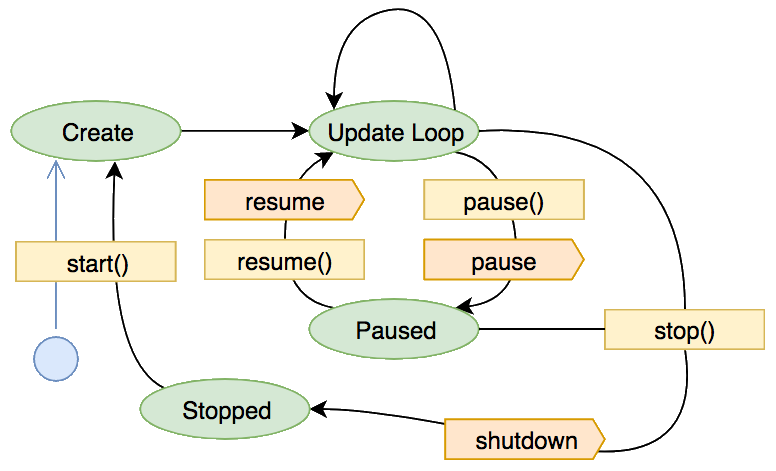
\includegraphics[width=0.8\textwidth]{figures/lifecycle}
    \caption{Scene Lifecycle [\ref{TODO}]}
    \label{fig:lifecycle}
\end{figure}

An interesting behavior is that once a scene has been shut down it is not garbage collected.
The scene can always be resumed by the start() method.
When this happens the three creation functions get called once more.
This means any state tracked in the scene class will be retained between a stopped state and the next create state.
Thus special care must be taken to set a known initial value on everything requiring one.
Especially when loading/creating objects outside the preloader (animations, tweens, audiofiles, etc.).

Scenes here have 5 functions:

\begin{itemize}
    \item \textbf{constructor()}: Run 1 time.
    \item \textbf{init()}: Run 1 time. Initialization of fields and passed on data by other scenes.
    \item \textbf{preload()}: Run 1 time. Loads up all the assets inside the scene like images and audio.
    \item \textbf{create()}: Run 1 time. Position and display the assets that are already preloaded, animations, physics, etc.
    \item \textbf{update()}: Run 1 time per frame, takes care of everything related to the game logic.
\end{itemize}

\subsection{Managers}\label{subsec:managers}
In Phaser 3 managers are a global system.
Animations, scenes, images loaded/created within it are globally available to all game objects.
They share the base data while managing their own timelines.
This allows the definition of a single object once and its application to as many game objects as required.
So a game object can be called in an completely other and unrelated scene.
Examples for used managers in this work are:

\begin{itemize}
    \item \textbf{Scene Manager} (scene.scenes). Contains all scenes of the game once created.
    \item \textbf{Texture Manager} (scene.textures). Contains all textures once loaded.
    \item \textbf{Audio Manager} (scene.sound). Contains all audio files once loaded.
    \item \textbf{Data Manager} (scene.data). Shared data manager.
    An event (listenable) is triggered when an event is stored/changed.
    \item \textbf{Cache Manager} (scene.cache). Contains all special files once loaded.
    \item \textbf{Animation Manager} (scene.anims). Contains all animations once created.
    \item \textbf{Tween Manager} (scene.tweens). Contains all tween objects once created.
    A Tween is able to manipulate the properties of one or more objects to any given value, based
    on a duration and type of ease.
\end{itemize}

\section{Object Generation}\label{sec:object-generation}
Our objects can have up to four properties with exactly one from each of the following categories:

\begin{itemize}
    \item \textbf{Geometrical shape} (square, triangle, circle, ellipse, rhombus, octagon)
    \item \textbf{Color} (yellow, orange, red, purple, green, blue)
    \item \textbf{Holes} or dots (one, two, three, four, five, six)
    \item \textbf{Filling} (filled, striped, dotted)
\end{itemize}

All possible objects with one, three and four properties, are needed.

With a python script [\ref{lst:svggen}] scalable vector graphic (SVG) [\ref{TODO}] files are generated [\ref{lst:svgimagefile}].
After that they are converted to portable network graphic (PNG)[\ref{TODO}] files with the GNU image manipulation program (GIMP) [\ref{TODO}].
Additional image scaling and cropping is done for saving space and only displaying the actual image with as less empty space as possible around it.
With the imagemagick command mogrify [\ref{lst:mogrify}] the last step is easily applicable to all 1000+ images.

\begin{lstlisting}[style=TypeScript, caption={ImageMagick console command "mogrify"}, label={lst:mogrify}]
    mogrify -resize 50% -trim -repage *.png
\end{lstlisting}

\begin{lstlisting}[style=TypeScript, caption={SVG Generation}, label={lst:svggen}]
    ...
    imageString = imgStr(colordefault, colordark, square, circle, triangle, ellipse, octagon, rhombus, filling, one,
                         two, three, four, five, six)

    filename = colordefault + shape + number + fillingname

    with open("images/svg/" + filename + ".svg", "w+") as file:
        file.write(imageString)
        file.close()
    ...
\end{lstlisting}

\begin{lstlisting}[style=TypeScript, caption={SVG Image File}, label={lst:svgimagefile}]
    <?xml version="1.0" standalone="yes"?>

    <svg height="1000" width="1000" viewbox="0 0 1000 1000" xmlns="http://www.w3.org/2000/svg">
    <defs>
            <pattern id="stripe" patternUnits="userSpaceOnUse" width="20%" height="20%">
                <path stroke="aqua" stroke-linecap="butt" stroke-width="50" d="M -20 -20 l1000 1000"/>
                <path stroke="aqua" stroke-linecap="butt" stroke-width="50" d="M -20 180 l1000 1000"/>
                <path stroke="aqua" stroke-linecap="butt" stroke-width="50" d="M -20 -220 l1000 1000"/>

            </pattern>
            <pattern id="dotted" enable-background="true" patternUnits="userSpaceOnUse" width="15%" height="15%">
                <circle cx="30" cy="30" r="25" fill="aqua" />
                <circle cx="105" cy="105" r="25" fill="aqua" />
            </pattern>
            <style>
            .button {

            stroke-width:5;
            stroke:black;

            }
        </style>
        </defs>

     <g id="circle" display="none">
         <circle cx="500" cy="500" r="300" class="button" fill="blue"/>
         <circle cx="500" cy="500" r="300" class="button" fill="none"/>
         <circle cx="500" cy="500" r="250" class="button" fill="none"/>
     </g>

     <g id="square" display="inherit">
      <rect x="250" y="250" rx="20" ry="20" width="500" height="500" class="button" fill="blue"/>
      <rect x="250" y="250" rx="20" ry="20" width="500" height="500" class="button" fill="none"/>
      <rect x="300" y="300" rx="20" ry="20" width="400" height="400" class="button" fill="none"/>
     </g>

     <g id="triangle" display="none">
      <polygon points="500,50 113.4,700 886.6,700" stroke-linejoin="round" class="button" fill="blue" />
      <polygon points="500,50 113.4,700 886.6,700" stroke-linejoin="round" class="button" fill="none" />
      <polygon points="500,150 200,650 800,650" stroke-linejoin="round" class="button" fill="none"/>
     </g>

     <g id="ellipse" display="none">
      <ellipse cx="500" cy="500" rx="400" ry="250" class="button" fill="blue" />
      <ellipse cx="500" cy="500" rx="400" ry="250" class="button" fill="none" />
      <ellipse cx="500" cy="500" rx="350" ry="200" class="button" fill="none" />
     </g>
     <g id="octagon" display="none">
      <polygon points="400,250 600,250 750,400 750,600 600,750 400,750 250,600 250,400" stroke-linejoin="round" class="button" fill="blue" />
      <polygon points="400,250 600,250 750,400 750,600 600,750 400,750 250,600 250,400" stroke-linejoin="round" class="button" fill="none" />
      <polygon points="400,300 600,300 700,400 700,600 600,700 400,700 300,600 300,400" stroke-linejoin="round" class="button" fill="none"/>
     </g>

     <g id="rhombus" display="none">
      <polygon points="350,250 150,750 650,750 850,250" stroke-linejoin="round" class="button" fill="blue" />
      <polygon points="350,250 150,750 650,750 850,250" stroke-linejoin="round" class="button" fill="none" />
      <polygon points="390,300 230,700 620,700 770,300" stroke-linejoin="round" class="button" fill="none"/>
     </g>


     <g id="one" display="none">
      <circle cx="500" cy="500" r="40" stroke="black" fill="black"/>
     </g>

     <g id="two" display="none">
      <circle cx="570" cy="500" r="40" stroke="black" fill="black"/>
      <circle cx="430" cy="500" r="40" stroke="black" fill="black"/>
     </g>

    <g id="three" display="none">
      <circle cx="570" cy="560" r="40" stroke="black" fill="black"/>
      <circle cx="430" cy="560" r="40" stroke="black" fill="black"/>
      <circle cx="500" cy="440" r="40" stroke="black" fill="black"/>
     </g>

    <g id="four" display="none">
      <circle cx="570" cy="430" r="40" stroke="black" fill="black"/>
      <circle cx="430" cy="430" r="40" stroke="black" fill="black"/>
      <circle cx="570" cy="570" r="40" stroke="black" fill="black"/>
      <circle cx="430" cy="570" r="40" stroke="black" fill="black"/>
    </g>
    <g id="five" display="none">
      <circle cx="570" cy="430" r="40" stroke="black" fill="black"/>
      <circle cx="430" cy="430" r="40" stroke="black" fill="black"/>
      <circle cx="570" cy="570" r="40" stroke="black" fill="black"/>
      <circle cx="430" cy="570" r="40" stroke="black" fill="black"/>
      <circle cx="500" cy="500" r="40" stroke="black" fill="black"/>
    </g>

    <g id="six" display="none">
      <circle cx="570" cy="400" r="40" stroke="black" fill="black"/>
      <circle cx="430" cy="400" r="40" stroke="black" fill="black"/>
      <circle cx="570" cy="600" r="40" stroke="black" fill="black"/>
      <circle cx="430" cy="600" r="40" stroke="black" fill="black"/>
      <circle cx="430" cy="500" r="40" stroke="black" fill="black"/>
      <circle cx="570" cy="500" r="40" stroke="black" fill="black"/>
    </g>

    Sorry, your browser does not support inline SVG.
    </svg>

\end{lstlisting}

\section{Objects}\label{sec:objects}
\subsection{Object Storage}\label{subsec:object-storage}
Our objects are images with different properties.
These properties cannot be saved in the images itself.
for that reason the image path with the respective properties are stored in a easily accessible
"JavaScript Object Notation" (JSON) file.

\begin{lstlisting}[style=TypeScript, caption={geometrical\_objects.json}]
{
  "categories": [
    {
      "name": "cat1",
      "url": "color.png",
      "validElements": [
        {
          "name": "purple",
          "urls": [
            "purple1.png",
            "purple2.png",
            "purple3.png",
            "purple4.png",
            "purple5.png",
            "purple6.png"
          ]
        },
        ...
      ]
    },
    ...
  ],
  "images": [
    {
      "name": "purplesquareonefull.png",
      "cat1": "purple",
      "cat2": "square",
      "cat3": "one",
      "cat4": "full"
    },
    ...
  ]
}
\end{lstlisting}

\subsection{Object Display}\label{subsec:object-display}
Displaying just the image of an object without tweaking it a little can seem boring for the user in long term.
To add more diversity, objects gets a random rotation angle, size and position every time it is displayed/created.
Of course within certain predefined boundaries.

\subsection{Object Interaction}\label{subsec:object-interaction}
Whenever possible a generalization of the input code is used with every user-object interaction.
Instead of giving each object an event task, the global event task is fetched and the object via the event parameters.
This way the input interaction code is kept in one place and so less fragmented.

\begin{lstlisting}[style=TypeScript, caption={Input code}]
    ...
    this.input.on('dragstart', function(pointer, gameObject) {
        ...
    }, this);

    this.input.on('drag', function(pointer, gameObject, dragX, dragY) {
        ...
    }, this);

    this.input.on('dragend', function(pointer, gameObject, dropped) {
        ...
        if (!dropped ...) {
            ...
        }
    }, this);

    this.input.on('drop', function(pointer, gameObject, dropZone) {
        ...
    }, this);
    ...
\end{lstlisting}

\section{Score Storage}\label{sec:scorestorage}
The achieved score is saved in the local storage of the browser.
The local storage remains unchanged until it is cleared in the browser settings.
Thus the saved score is not lost on the same device until purposely deleted.
Before accessing the local storage it is checked if there even is a storage.

\begin{lstlisting}[style=TypeScript, caption={Storage access (scoreScene.ts)}]
    ...
    private saveScore(score: string): void {
        if (typeof(Storage) !== "undefined") {
            window.localStorage.setItem('phaser_score_' + this.previousScene, score);
        } else {
            console.log("Sorry! No Web Storage support...");
        }
    }
    ...
\end{lstlisting}

\begin{lstlisting}[style=TypeScript, caption={Storage access (levelMenuScene.ts)}]
    ...
    if (typeof(Storage) !== "undefined") {
        if(window.localStorage.getItem('phaser_score_' + this.buttonToSceneMap(gameObject.name))){
            if (reset) {
                window.localStorage.setItem('phaser_score_' + this.buttonToSceneMap(gameObject.name), score);
            } else {
                score = window.localStorage.getItem('phaser_score_' + this.buttonToSceneMap(gameObject.name));
            }
        }
    } else {
        console.log("Sorry! No Web Storage support...");
    }
    ...
\end{lstlisting}

\section{Introduction Animation Generation}\label{sec:introduction-animation-generation}
To produce animated instruction for the task later on,
the screen is recorded with the Open Broadcaster Software (OBS) Studio [\ref{TODO}] while someone is playing the game.
Parts of the final video are then taken for the respective scenes and converted into single pictures.
These single pictures are saved in one picture (called spreadsheet [\ref{fig:spreadsheet}]).
The Phaser framework animates those spreadsheets.

Is is important to note, that different devices have a different limit for the resolution of images.
Tablets seem to have the lowest, namely 4096x4096 pixels [\ref{TODO}].
The spreadsheet images are scaled down for that reason.

\begin{figure}[H]
    \centering
    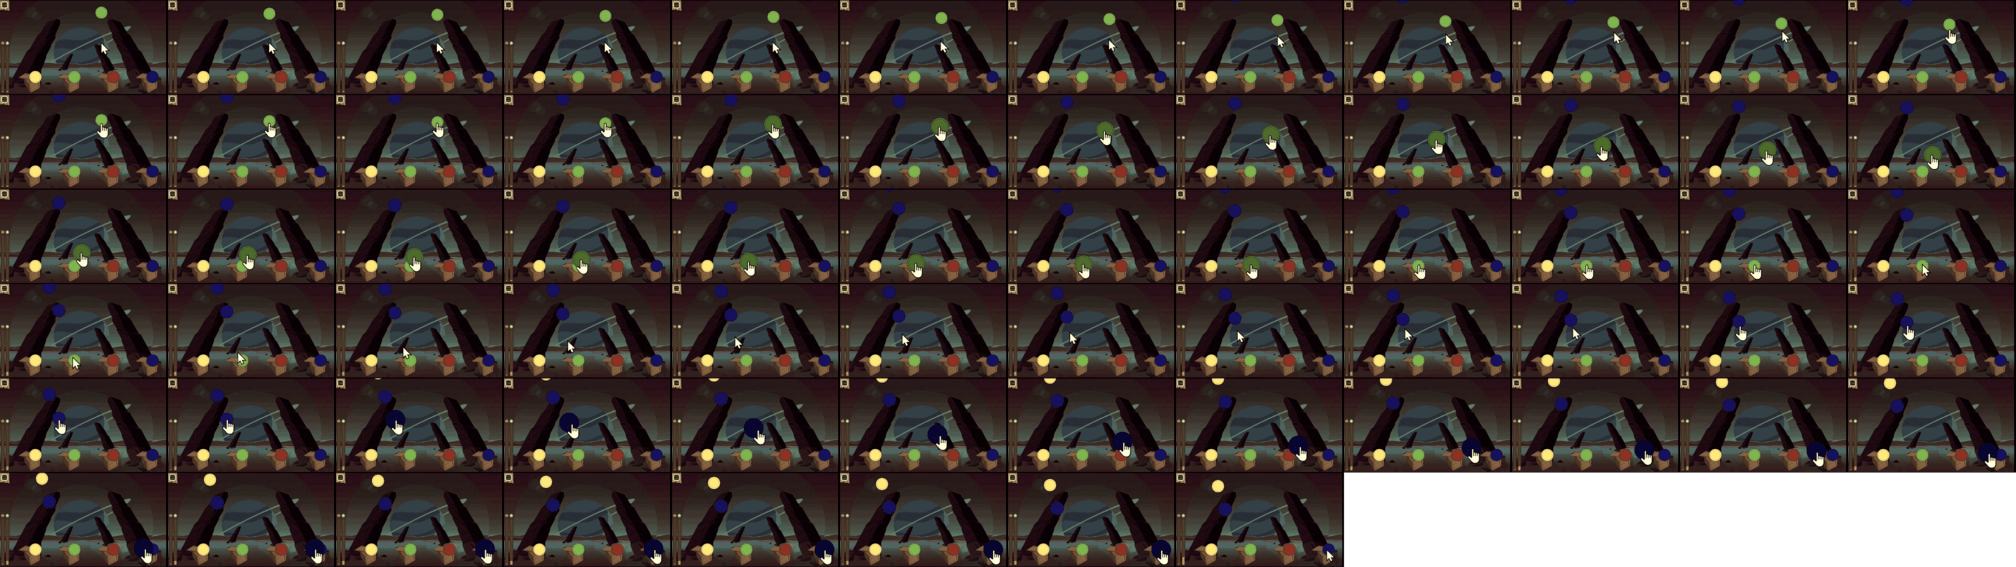
\includegraphics[width=1\textwidth]{figures/spreadsheet}
    \caption{Example: Spreadsheet}
    \label{fig:spreadsheet}
\end{figure}

\section{Concept of the Learning Environment}\label{sec:concept-of-the-learning-environment}
Through the given boundary conditions and requirements the environment is split into multiple parts/scenes.

\subsection{Drop Down Menu}\label{subsec:drop-down-menu}
Throughout the whole experience, the user can open a menu with a button.
This button is always visible.
Once the menu is open, the user may close the menu and return to the current scene,
exit the current scene and return to the level menu and go into fullscreen and back.
The current scene is paused while the menu is open as it can be distracting for the user,
if suddenly something pops up and covers parts of the visible and running scene.

\subsection{Welcome Screen}\label{subsec:welcome-screen}
The welcome screen is the starting point of the user experience.
Through this screen the user is greeted by showing the name of the game.
Through a click he may commence to the level menu.

\subsection{Level Menu}\label{subsec:level-menu}
In the level menu, the user is able to choose between different levels and games and can access the object summary.
Through the stars below each button the user can track his progress/score.
The progress can be resetted by the reset button.

\subsection{Object Summary}\label{subsec:object-summary}
The Object summary allows the user to get a feeling for all the different properties an object can have.
For that reason the number of objects per category is restricted to five, as there are over 1000 different objects.
Objects are draggable and sortable by each category with a click on a respective button.

\subsection{Sorting with one Category}\label{subsec:sorting-with-one-category}
Here the user has to sort the static objects with one category by the given category.
As the user should be able to experience all categories, they are split into different levels.
Each level represents a category.
For motivation, the user can track his progress.
The Progress is defined by objects sorted the right and the wrong way.

The amount of objects to sort, as well as the amount of properties of the category
is randomly selected each time you start the game.

\subsection{Sorting with one category under difficult conditions}\label{subsec:sorting-with-one-category-under-difficult-conditions}
Here the user has to sort falling objects with one category by the given category.
As the user should be able to experience all categories, they are split into different level.
Each level represents a category.
For motivation, the user can track his progress.
The progress is defined by objects missed, sorted the right and the wrong way.
To make the task harder, dummy objects are added.
Those objects look similar to the original ones but with a succinct characteristic.
There are no negative points for missing such an object but negative points for sorting them in any way.

For more diversity, the amount of falling objects to sort, as well as the amount of properties of the category
is randomly selected each time you start the game.

\subsection{Sorting with restricted space}\label{subsec:sorting-with-restricted-space}
In this scene the user has to sort a given number of objects with all properties shown into boxes with limited space.
The objects in one box must have at least one property in common and
can be put into the box and taken out an infinite amount of times.

To make the game more difficult, this level is split into two.
The first level has boxes with the size 6, 4, 2 and the second one boxes with the size 6, 5, 4.

\subsection{Object pairing - easy version}\label{subsec:object-pairing---easy-version}
In this game, twelve objects with three categories are shown.
the user has to select three objects which have to fulfil the following.
For each category (color, shape and number of holes/dots) one of the following conditions has to hold:
\begin{itemize}
    \item They must be the same (blue, blue, blue)
    \item They must be completely different (square, triangle, circle)
\end{itemize}

\begin{figure}[H]
    \centering
    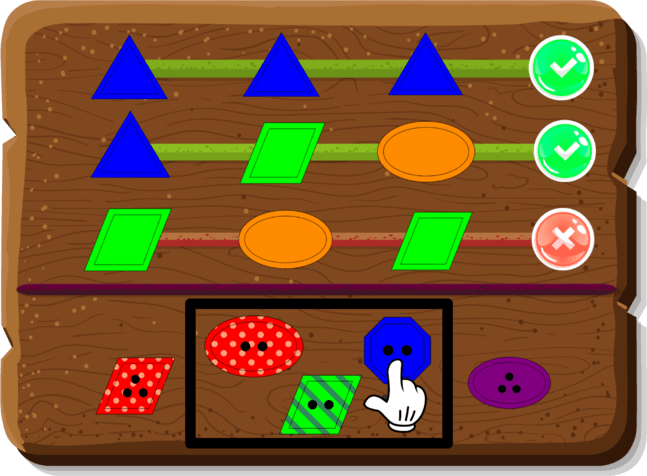
\includegraphics[width=0.8\textwidth]{figures/setexample}
    \caption{Example: Matching Set}
    \label{fig:setexample1}
\end{figure}

If the user needs help, there is a helper bar which can be accessed by a button with a question mark on it.
The helper bar shows which categories fulfil the conditions and which do not
by coloring the category symbols on the bar in green or red.

The game is time limited. The remaining time is shown by a bar.
If you select three objects which fulfil the conditions, more time will be added.
After a set amount of correct selected objects, the game will end.

If there are no three objects that fulfil the conditions, the playfield will be generated anew.

\subsection{Object pairing - normal version}\label{subsec:object-pairing---normal-version}
In this game, twelve objects with four categories are shown.
the user has to select three objects which have to fulfil the following.
For each category (color, filling, shape and number of holes/dots) one of the following conditions has to hold:
\begin{itemize}
    \item They must be the same (blue, blue, blue)
    \item They must be completely different (square, triangle, circle)
\end{itemize}

\begin{figure}[H]
    \centering
    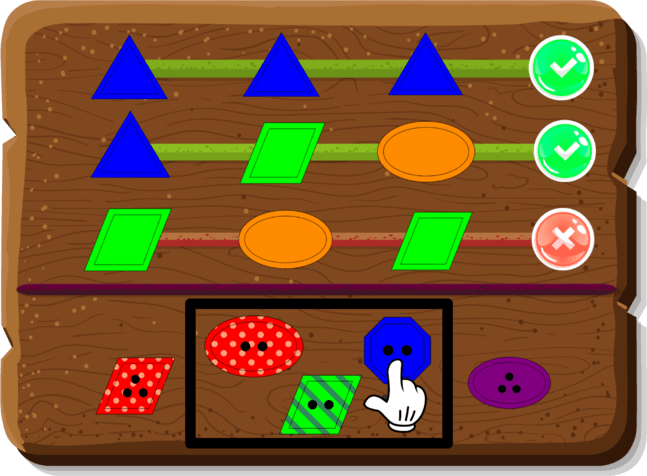
\includegraphics[width=0.8\textwidth]{figures/setexample}
    \caption{Example: Matching Set}
    \label{fig:setexample2}
\end{figure}

If the user needs help, there is a helper bar which can be accessed by a button with a question mark on it.
The helper bar shows which categories fulfil the conditions and which do not
by coloring the category symbols on the bar in green or red.

The game is time limited. The remaining time is shown by a bar.
If you select three objects which fulfil the conditions, more time will be added.
After a set amount of correct selected objects, the game will end.

If there are no three objects that fulfil the conditions, the playfield will be generated anew.

\subsection{Score Screen}\label{subsec:score-screen}
After a task has been completed, there is going to be a score.
This score is represented here with a displayed number of stars.
The minimum of starts is zero and the maximum is three.
If the user is unhappy with his results, he can replay the game by clicking on the replay button.

\subsection{Introduction}\label{subsec:introduction}
Before each game starts, a sample animation of the task beforehand is being shown.
The current scene is paused in the meantime, so that the user has enough time to find out what he has to do.

\section{Code structure of the learning environment}\label{sec:code-structure-of-the-learning-environment}
Our learning environment consists of different scenes each one inheriting the base scene.
The following subsections won't contain the whole code as some parts are trivial to understand.
Instead a summary of the scenes purpose and crucial parts are shown and explained.

The full code can be accessed in the appendix.

\begin{figure}[H]
    \centering
    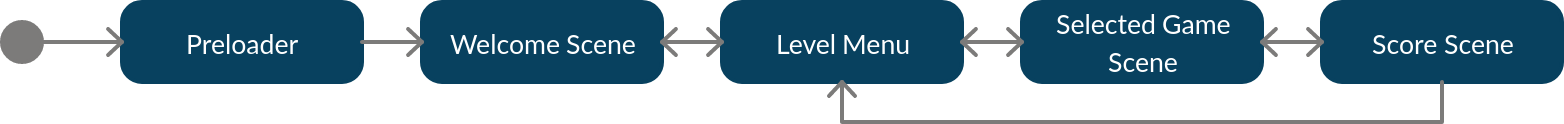
\includegraphics[width=1\textwidth]{figures/statediagram}
    \caption{Scene Statediagram}
    \label{fig:statediagram}
\end{figure}

\subsection{BaseScene}\label{subsec:basescene}
This scene contains methods and fields which are necessary in multiple scenes
(e.g. the scene transition, identifier of the scene, ...).

The transition is a mask in the form of a circle laid over a black rectangle.
Masks have to be applied to every object they have to mask.
So a simple solution was to lay a black rectangle over the whole scene and mask it.
The animated transition is created by increasing or decreasing the radius of the circle
mask according to the wanted animation (IN/OUT).

\begin{lstlisting}[style=TypeScript, caption={BaseScene.ts}]
    ...
    private transitionInit(): void {
        // Shape of the graphical transition
        const circle: Phaser.GameObjects.Graphics = this.add.graphics();

        // Shape of the screen
        const rectangle: Phaser.GameObjects.Rectangle = this.add.rectangle(0, 0, this.cameras.main.width, this.cameras.main.height, 0x000000);

        // Define circle as the mask
        const mask: Phaser.Display.Masks.GeometryMask = circle.createGeometryMask();

        circle.setPosition(this.cameras.main.width / 2, this.cameras.main.height / 2);
        circle.fillCircle(0, 0, 0.1);
        circle.setDepth(0);

        mask.setInvertAlpha(true);

        rectangle.setDepth(1);
        rectangle.setOrigin(0, 0);
        rectangle.setMask(mask);

        circle.fillCircle(0, 0, 0.1);

        this.transition = [circle, rectangle];
    }
\end{lstlisting}

\subsection{PreloadAssets}\label{subsec:preloadassets}
In the method "preload()" the files used later on can be loaded into the respective managers/cache.
If files are loaded in a method outside of the preload method, the loader has to be started manually (in the code).
Now every asset loaded this way has a unique identifier and can be used in future scene
as long as it is not removed explicitly.
The asset can as such be loaded into the managers/cache in every scene,
so that only the actual used assets are loaded.
The advantage of this is that you can save time and storage.
But the disadvantage is that you have to be connected to the internet the whole time.
Should the connection be severed for only a short time, objects might not be displayed correctly.
With a "preload" scene in the beginning all available assets are loaded,
so that after the longer loading time the game can run fluently,
without problems and most importantly without a connection to the internet.

The attributes and path of objects in the imported json file [REFERENCE TO EXPLANATION TOP]
can be accessed by filename.["fieldname"] or filename.fieldname:

\begin{lstlisting}[style=TypeScript, caption={Example json file access}]
    ...
    for (let category of loadedJsonObjectFile['categories']) {
        console.log("URL: " + category['url']);
        console.log("Name: " + category['validElements']['name']);
        console.log("ValidElement urls: " + category['validElements']['urls']);
    }

    for (let image of loadedJsonObjectFile['images']) {
        console.log("Name: " + image.name);
        console.log("Cat1: " + image.cat1);
        ...
    }
    ...
\end{lstlisting}

The way the objects files are preloaded into the respective managers is shown below.

\begin{lstlisting}[style=TypeScript, caption={preloadAsset.ts}]
    ...
    private preload(): void {
        this.load.setPath('assets/geometrical_objects/');
        this.load.json('objects', 'geometrical_objects.json');
        ...
    }
    ...
    private preLoadImages(): void {
        // Load category and object images
        const jsonObject: any = this.cache.json.get('objects');

        for (let category of jsonObject['categories']) {
            this.load.setPath('assets/geometrical_objects/categories/');
            this.load.image(category['name'], category['url']);

            this.load.setPath('assets/geometrical_objects/images/');
            for (let property of category['validElements']) {
                for (let url of property['urls']) {
                    this.load.image(url, url);
                }
            }
        }

        for (let image of jsonObject['images']) {
            this.load.image(image['name'], image['name']);
        }
        ...
    }
    ...
\end{lstlisting}

\subsubsection{Image Game Objects}
Instead of representing an image as a normal image in game, sprites, a special texture, is used.
A sprite game object can display both static and animated images in your game.
They have input events, additional functions, fields and physics bodies.
The main difference between a sprite and an image game object is that you cannot animate images.

\subsection{DropDownMenu}\label{subsec:dropdownmenu}
In this scene the drop down menu is created.
This scene is never stopped and is always on top of other scenes.

The following code in every other scene ensures this:
\begin{lstlisting}[style=TypeScript, caption={Send current scene to back}]
    ...
    create(): void {
        this.game.scene.sendToBack(this.getKey());
        ...
    }
    ...
\end{lstlisting}

As the drop down animation takes time, it was necessary to create a boolean field as a lock.
This ensures that the closing and opening animation won't interfere with each other.
The lock is freed after the completion of an event/animation.

\begin{lstlisting}[style=TypeScript, caption={Lock aquiring and freeing}]
    ...
    if (!this.lock) {
        this.lock = true;
        ...
    }
    ...
    onComplete: () => this.lock = false;
    ...
\end{lstlisting}

While the menu is down/open, the current scene has to be paused.
This is achieved by accessing the other scene by fetching the key of the only other active scene and pausing it.
Important to note is, that the last started/activated scene is at position 0 in the array of all active scenes.
\begin{lstlisting}[style=TypeScript, caption={Fetching current active scene}]
    ...
    const key_paused_scene: string = this.game.scene.getScenes(true)[0].key;
    this.game.scene.pause(key_paused_scene);
    this.key_paused_scene = key_paused_scene;
    ...
\end{lstlisting}

The same trick is used for closing all current scenes when exiting (without the dropDownMenu Scene).

\subsection{WelcomeScene}\label{subsec:welcomescene}
A blinking finger is added to the screen so that the user knows that he can advance by clicking on the screen.

\subsection{LevelMenuSceneScene}\label{subsec:levelmenuscenescene}
Levels with the same difficulty are distinguished by numbers from one to four.
Levels with another difficulty are distinguished by images of monsters with different level of spookiness.

\begin{figure}[H]
    \centering
    
\includegraphics[width=0.2\textwidth]{figures/easylevelicon}
    \caption{Easy Level Icon}
    \label{fig:easylevelicon}
\end{figure}

\begin{figure}[H]
    \centering
    
\includegraphics[width=0.2\textwidth]{figures/mediumlevelicon}
    \caption{Medium Level Icon}
    \label{fig:mediumlevelicon}
\end{figure}

\begin{figure}[H]
    \centering
    
\includegraphics[width=0.2\textwidth]{figures/hardlevelicon}
    \caption{Hard Level Icon}
    \label{fig:hardlevelicon}
\end{figure}

\subsection{IntroScene}\label{subsec:introscene}
To pause the current scene and still play the introduction animation, a separate scene is necessary.
Each time an intro has to be played, the intro scene is started anew.
The current scene is pauses itself when the intro scene is started and the name/key/identifier
of the paused scene is given to the intro scene.
That way the intro scene can resume the paused scene and then stop itself.

The respective intro material is selected via the name/key/identifier of the paused scene.

\subsection{SortingScene}\label{subsec:sortingscene}
To sort the displayed objects by their respective subcategory by clicking on one of the category buttons,
random coordinates are needed dependant on the screen size and object size.
\begin{lstlisting}[style=TypeScript, caption={returnQuad() (sortingScene.ts)}]
    ...
    private returnQuad(quadrant: number, quadrantType: number): number[] {
        let ret: number[] = null;
        ...
        const leftOffsite: number = 100;
        const rightOffsite: number = 0;
        const topOffsite: number = 0;
        const bottomOffsite: number = 100;

        // Has entries dependant of
        const horizontal: number[] = [];

        // Has numberOfLines + 1 entries
        const vertical: number[] = [];

        horizontal.push(leftOffsite);

        vertical.push(topOffsite);

        switch (quadrantType) {
            case 3: {
                horizontal.push(leftOffsite + (this.cameras.main.width - leftOffsite - rightOffsite) / 3);
                horizontal.push(leftOffsite + (this.cameras.main.width - leftOffsite - rightOffsite) * 2 / 3);
                break;
            }
            case 4: {
                horizontal.push(leftOffsite + (this.cameras.main.width - leftOffsite - rightOffsite) / 2);
                vertical.push(topOffsite + (this.cameras.main.height - topOffsite - bottomOffsite) / 2);
                break;
            }
            case 6: {
                horizontal.push(leftOffsite + (this.cameras.main.width - leftOffsite - rightOffsite) / 3);
                horizontal.push(leftOffsite + (this.cameras.main.width - leftOffsite - rightOffsite) * 2 / 3);
                vertical.push(topOffsite + (this.cameras.main.height - topOffsite - bottomOffsite) / 2);
                break;
            }
            default: {
                break;
            }
        }

        horizontal.push(this.cameras.main.width - rightOffsite);
        vertical.push(this.cameras.main.height - bottomOffsite);

        switch (quadrantType) {
            case 3: {
                ret = [Phaser.Math.RND.between(horizontal[quadrant] + spriteSizeHalf, horizontal[quadrant + 1] - spriteSizeHalf), Phaser.Math.RND.between(vertical[0] + spriteSizeHalf + this.cameras.main.height / 8, vertical[1] - spriteSizeHalf - this.cameras.main.height / 8)];
                break;
            }
            case 4: {
                if (quadrant < 2) {
                    ret = [Phaser.Math.RND.between(horizontal[quadrant] + spriteSizeHalf, horizontal[quadrant + 1] - spriteSizeHalf), Phaser.Math.RND.between(vertical[0] + spriteSizeHalf, vertical[1] - spriteSizeHalf)];
                } else {
                    ret = [Phaser.Math.RND.between(horizontal[quadrant \% 2] + spriteSizeHalf, horizontal[(quadrant \% 2) + 1] - spriteSizeHalf), Phaser.Math.RND.between(vertical[1] + spriteSizeHalf, vertical[2] - spriteSizeHalf)];

                }
                break;
            }
            case 6: {
                if (quadrant < 3) {
                    ret = [Phaser.Math.RND.between(horizontal[quadrant] + spriteSizeHalf, horizontal[quadrant + 1] - spriteSizeHalf), Phaser.Math.RND.between(vertical[0] + spriteSizeHalf, vertical[1] - spriteSizeHalf)];
                } else {
                    ret = [Phaser.Math.RND.between(horizontal[quadrant \% 3] + spriteSizeHalf, horizontal[(quadrant \% 3) + 1] - spriteSizeHalf), Phaser.Math.RND.between(vertical[1] + spriteSizeHalf, vertical[2] - spriteSizeHalf)];
                }
                break;
            }
            default: {
                break;
            }
        }
        return ret;
    }
\end{lstlisting}

\subsection{PropertySortingScene}\label{subsec:propertysortingscene}
To specify the difficulty level, two fields are needed:
\begin{lstlisting}[style=TypeScript, caption={Level fields (propertySortingScene.ts)}]
    ...
    private setCat: number;
    ...
    private infinite: boolean;
    ...
\end{lstlisting}

In contrast to other scenes, objects must have the type Phaser.Physics.Arcade.Sprite as only arcade sprites have the
possibility of an acceleration in a direction.

As additional visual feature objects get a random spin velocity and the time a object spawns gets shorter over time.

\subsection{RestrictedSortingScene}\label{subsec:restrictedsortingscene}
To check if objects in the same box have some property in common,
the four properties of a object are taken as a list of strings and intersected with the other list of strings from other
objects in the same box.
If finally there is no empty list, the objects have some property in common and thus this is a valid solution for one box.
Which one does not matter to us in this case.
In this way, it is possible that there are multiple solutions which were not intended but also correct.

\begin{lstlisting}[style=TypeScript, caption={equalityCheck (restrictedSortingScene.ts)}]
    ...
        private equalityCheck(gameObject: Phaser.GameObjects.Sprite, dropZone: Phaser.GameObjects.Zone): boolean {
        ...
        let mergeArray: any[] = [];
        ...
        for (let cat of this.jsonObject['categories']) {
            mergeArray = [...mergeArray, ...cat['validElements']];
        }
        mergeArray.forEach((element, index, array) => array[index] = element.name);
        ...
        [...this.objZoneMap.filter((element, index) => this.zoneObjMap[index].name === dropZone.name), gameObject].forEach(function (element) {
            mergeArray = mergeArray.filter((x) => element.getData('properties').includes(x));
        });
        ...
        return (mergeArray.length > 0);
    }
    ...
\end{lstlisting}

\subsection{GameScene}\label{subsec:gamescene}
In the game scene three marked objects are checked for equality
if the checker was not already run for those three objects.

\begin{lstlisting}[style=TypeScript, caption={update (gameScene.ts)}]
    update(time: number): void {
        ...
        if (!this.checked && this.arrayMarked.getLength() >= 3) {
            this.checked = true;
            ...
        }
        ...
        if (timedata <= 0) {
            this.checked = true;

            ...
        } else {
            timedata -= this.timedataStepsize;
            this.timefluid.setData('timeY', timedata);
            this.timefluid.setScale(this.timefluid.getData('timeX'), timedata);
        }
    }
\end{lstlisting}

As 'gameMax' is calculated with a quotient there is a rounding error in the floating point arithmetic.
To even this error we add or subtract epsilon, the maximum relative error of the rounding procedure.

\begin{lstlisting}[style=TypeScript, caption={updateProgressbar (gameScene.ts)}]
    ...
    if (this.points >= this.gamefluid.getData('gameMax') - Phaser.Math.EPSILON) {
        ...
    }
\end{lstlisting}

To mark the helpers menu icons the checkEquality method is modified
with a boolean to mark the icons while executing the check.

\begin{lstlisting}[style=TypeScript, caption={checkEquality (gameScene.ts)}]
    ...
    private checkEquality(sprite1: Phaser.GameObjects.GameObject, sprite2: Phaser.GameObjects.GameObject, sprite3: Phaser.GameObjects.GameObject, inGame: boolean): boolean {
        if (sprite1 instanceof Phaser.GameObjects.Sprite &&
            sprite2 instanceof Phaser.GameObjects.Sprite &&
            sprite3 instanceof Phaser.GameObjects.Sprite
        ) {
            // Return value
            let replaceObjects: boolean = true;

            for (let categoryIndicator of this.arrayCategory.getChildren()) {

                // Make sure your objects are sprites
                if (categoryIndicator instanceof Phaser.GameObjects.Sprite) {

                    // Clear tint
                    categoryIndicator.clearTint();

                    if (
                        sprite1.getData(categoryIndicator.name) === sprite2.getData(categoryIndicator.name) &&
                        sprite2.getData(categoryIndicator.name) === sprite3.getData(categoryIndicator.name) &&
                        sprite1.getData(categoryIndicator.name) === sprite3.getData(categoryIndicator.name)
                    ) {
                        if (inGame) {
                            categoryIndicator.setTintFill(0x00dd00);
                        }
                    } else if (
                        !(sprite1.getData(categoryIndicator.name) === sprite2.getData(categoryIndicator.name)) &&
                        !(sprite2.getData(categoryIndicator.name) === sprite3.getData(categoryIndicator.name)) &&
                        !(sprite1.getData(categoryIndicator.name) === sprite3.getData(categoryIndicator.name))
                    ) {
                        if (inGame) {
                            categoryIndicator.setTintFill(0x00dd00);
                        }
                    } else {
                        if (replaceObjects) {
                            replaceObjects = false;
                        }
                        if (inGame) {
                            // Mark category as red
                            categoryIndicator.setTintFill(0xdd0000);
                        }
                    }
                }
            }
            return replaceObjects;
        }
    }
\end{lstlisting}

To add another small gamification element in the form of a mini reward to the game, every time the user finds a matching
pair, some additional is added to the timer. So the user is even more motivated find pairs even faster.

\begin{lstlisting}[style=TypeScript, caption={updateProgressbar (gameScene.ts)}]
    ...
    let timedata: number = this.timefluid.getData('timeY');
    timedata += this.timedataStepsize * 5000;
    if (timedata > this.timefluid.getData('timeYMax')) {
        timedata = this.timefluid.getData('timeYMax');
    }
    ...
\end{lstlisting}

As frustrating as it is to find no matching pair,
it is ensured that there is at least one possible pair every time a new object is added.

\begin{lstlisting}[style=TypeScript, caption={INSERT (gameScene.ts)}]
    ...
    private rebuildDisplayedObjects(): void {
        ...
        for (let card of this.arrayDisplayed.getChildren()) {
            if (card instanceof Phaser.GameObjects.Sprite) {
                card.setVisible(false);
                this.arrayStack.add(card);
            }
        }

        this.arrayDisplayed.clear(false, false);

        this.initObjects();
    }
    ...
\end{lstlisting}

\subsection{ScoreScene}\label{subsec:scorescene}
The most important and special part in the score scene is the way the score is saved,
as explained in this \hyperref[ref:scorestorage]{section}.

\section{Final Look of the Learning Environment}\label{sec:final-look-of-the-learning-environment}
This section contains the final look of the learning environment.

\begin{figure}[H]
    \centering
    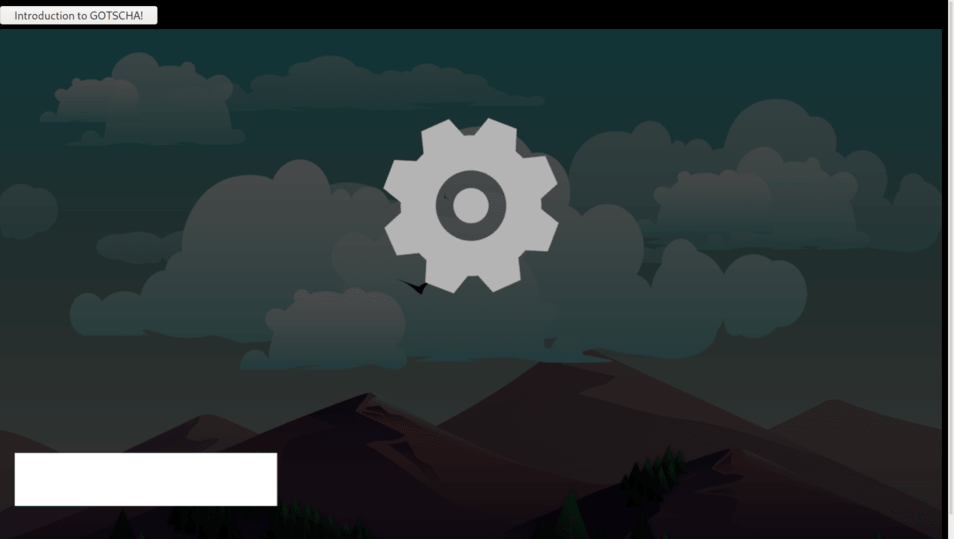
\includegraphics[width=1\textwidth]{figures/loadingscreen}
    \caption{Loading Screen}
    \label{fig:loadingscreen}
\end{figure}

\begin{figure}[H]
    \centering
    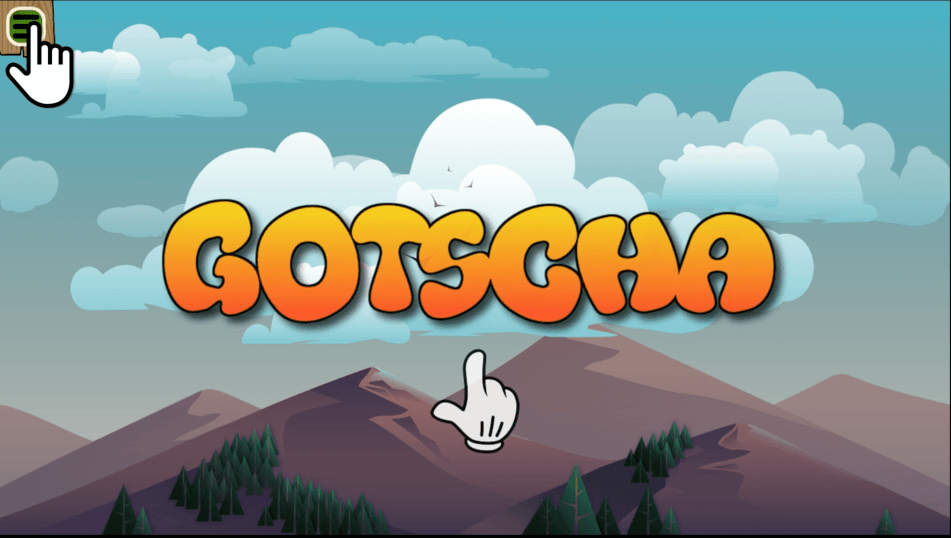
\includegraphics[width=1\textwidth]{figures/welcomescreen}
    \caption{Title Screen}
    \label{fig:titlescreen}
\end{figure}

\begin{figure}[H]
    \centering
    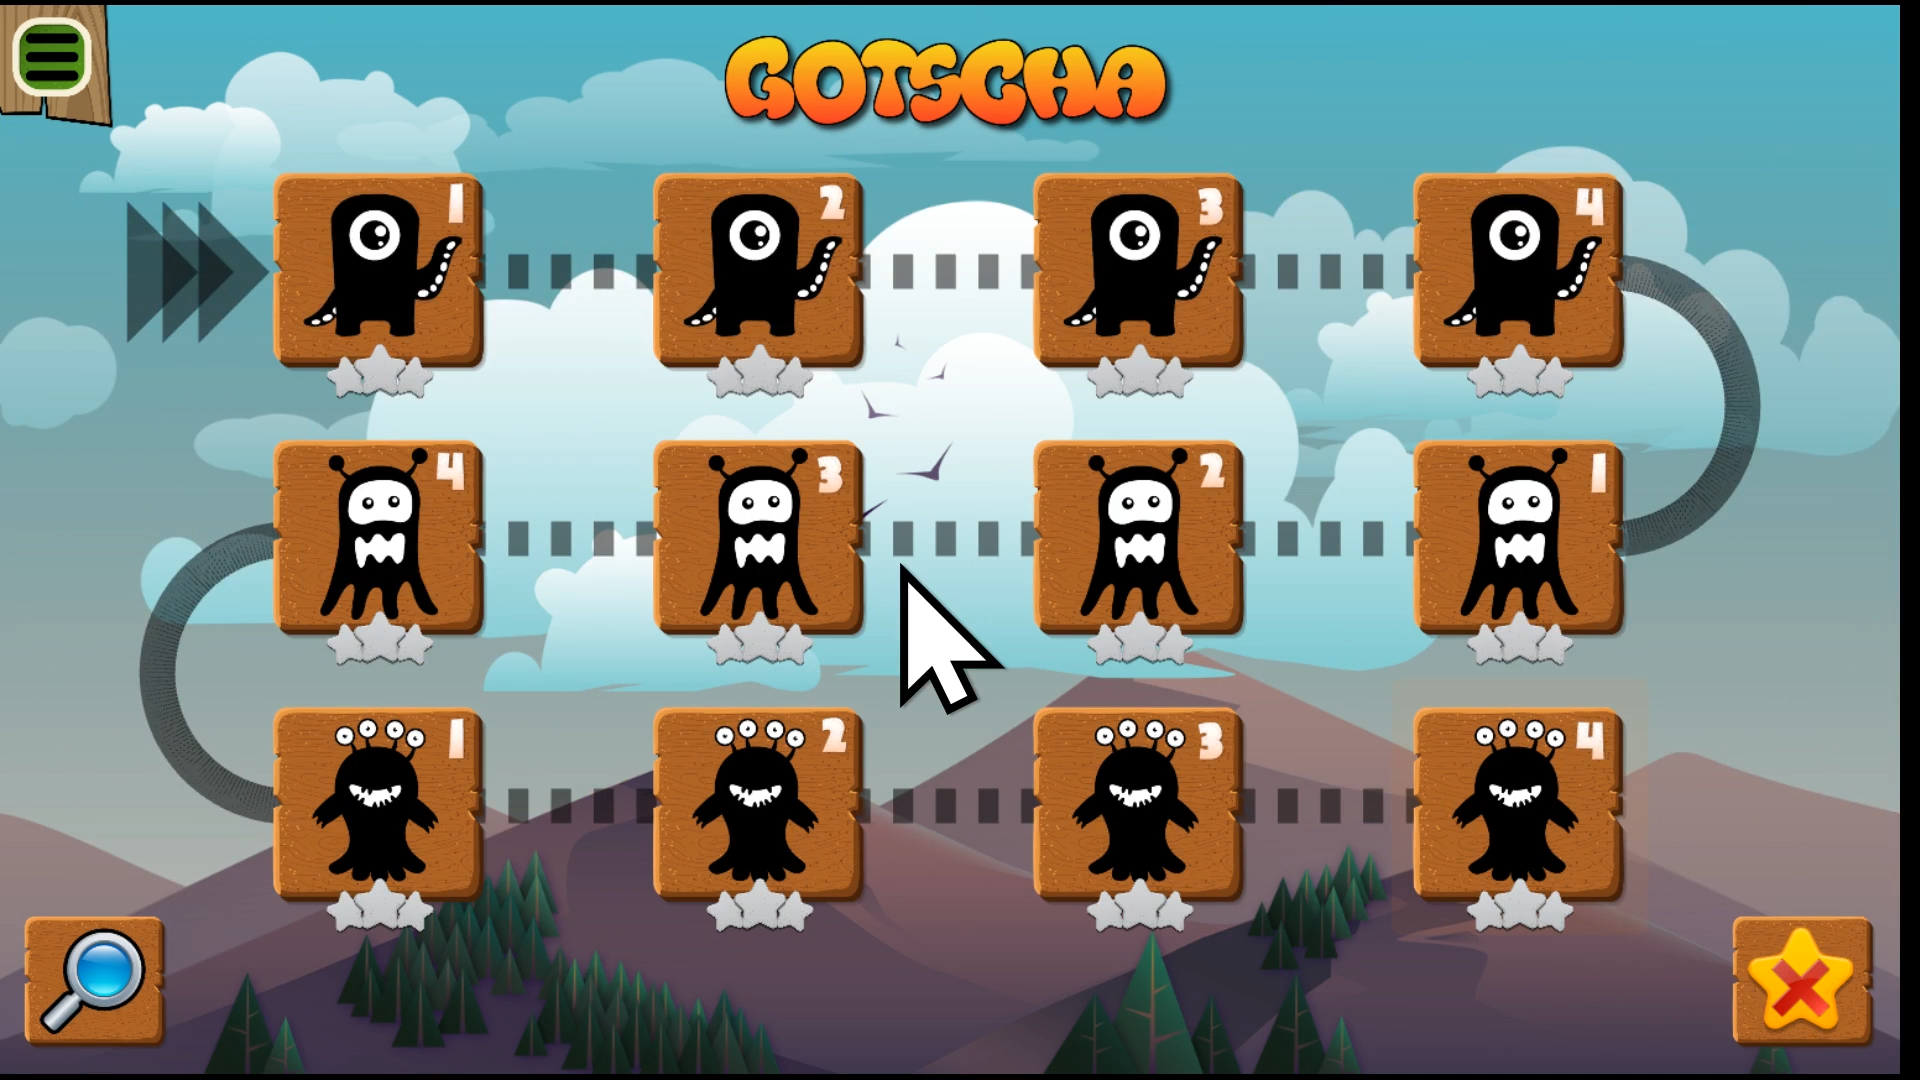
\includegraphics[width=1\textwidth]{figures/levelmenu}
    \caption{Level Menu}
    \label{fig:levelmenu}
\end{figure}

\begin{figure}[H]
    \centering
    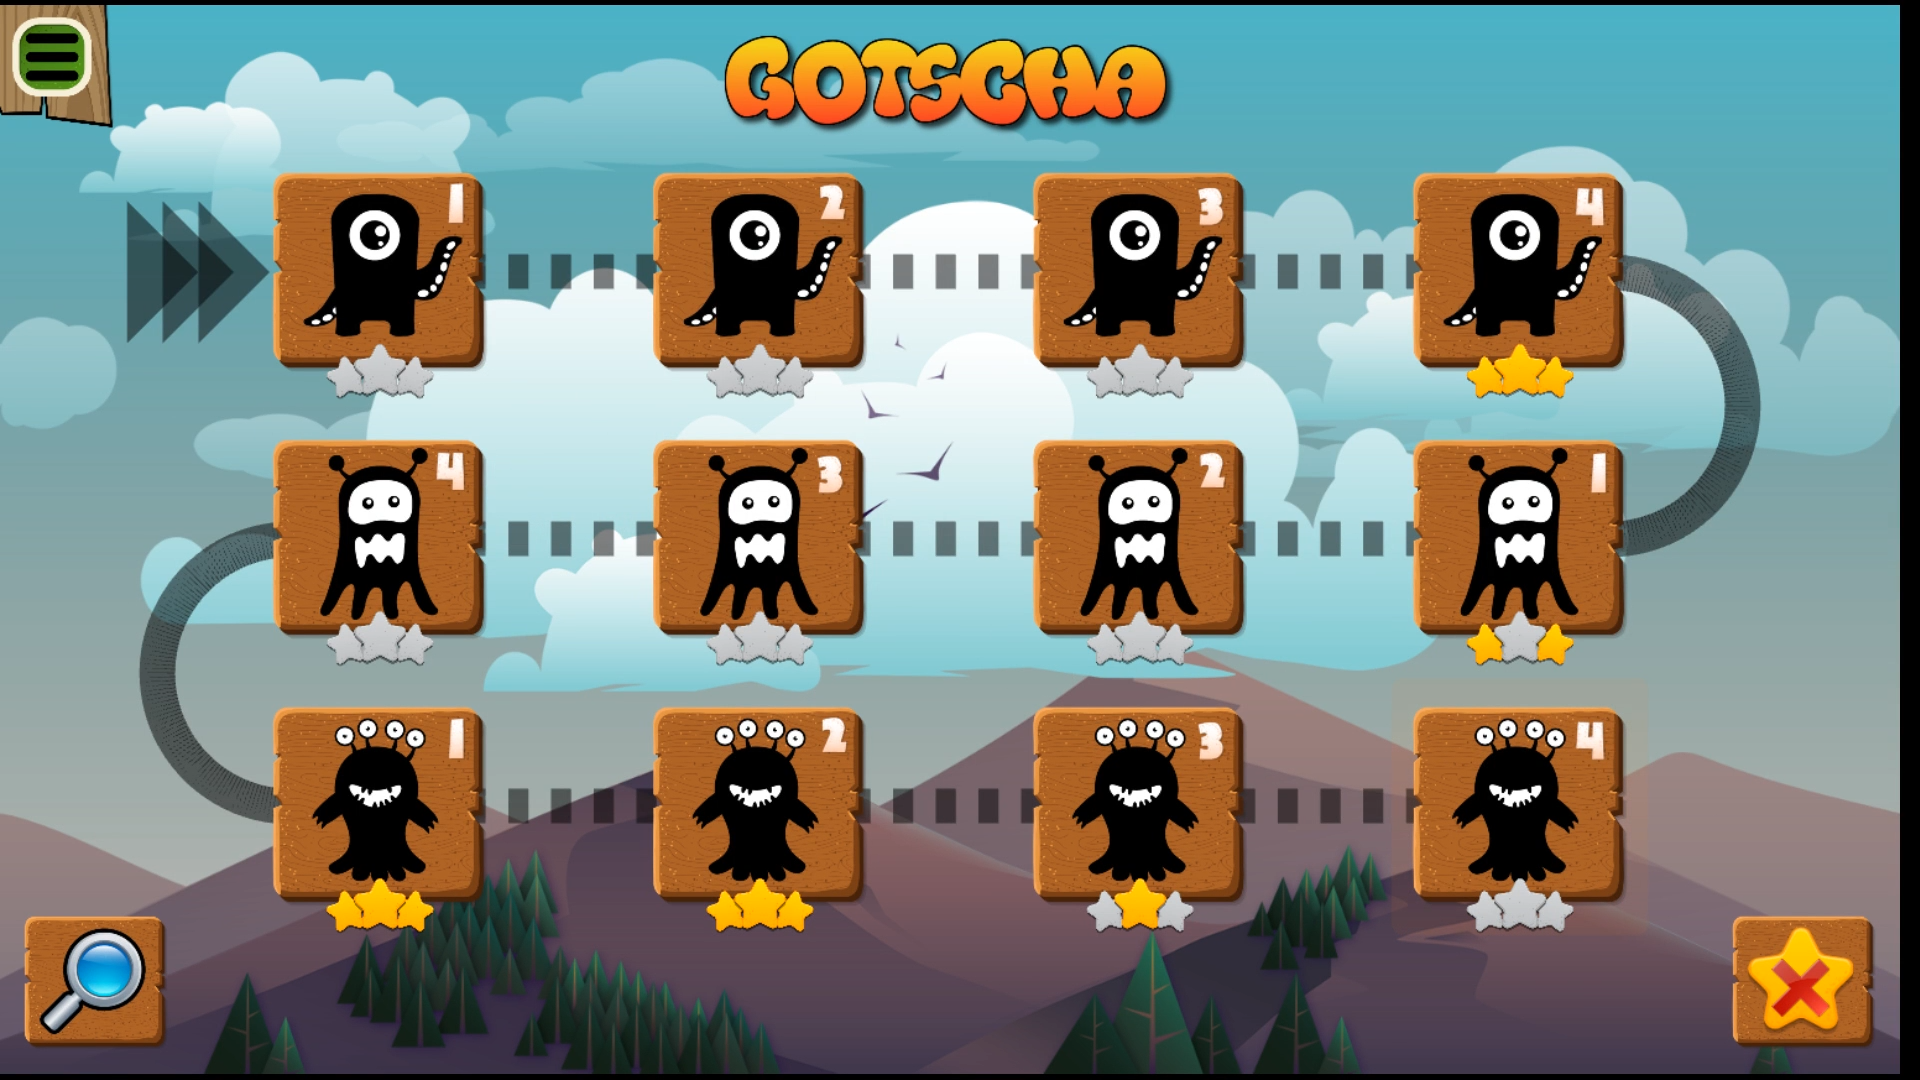
\includegraphics[width=1\textwidth]{figures/levelmenustars}
    \caption{Level Menu showing Stars}
    \label{fig:levelmenustars}
\end{figure}

\begin{figure}[H]
    \centering
    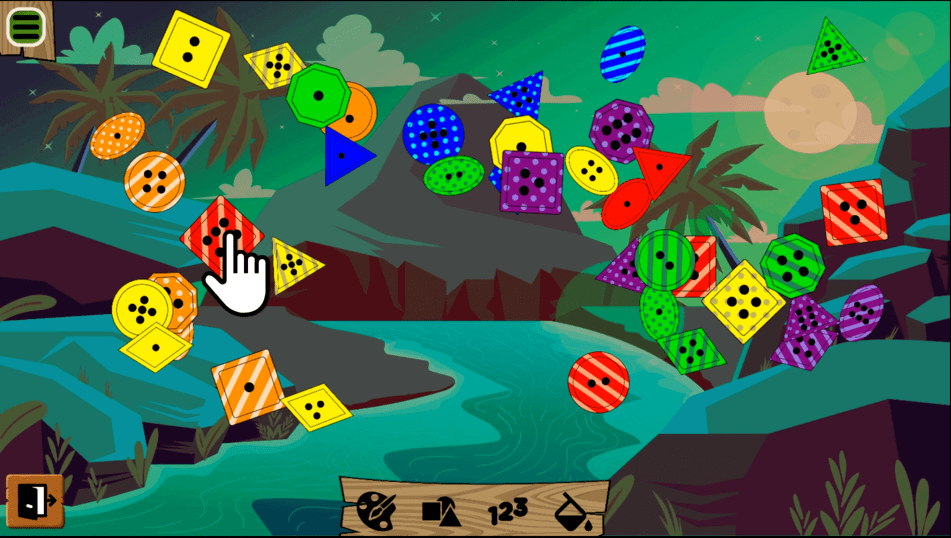
\includegraphics[width=1\textwidth]{figures/sortingscene1}
    \caption{Sorting Scene Category Mixture}
    \label{fig:sortingscene1}
\end{figure}

\begin{figure}[H]
    \centering
    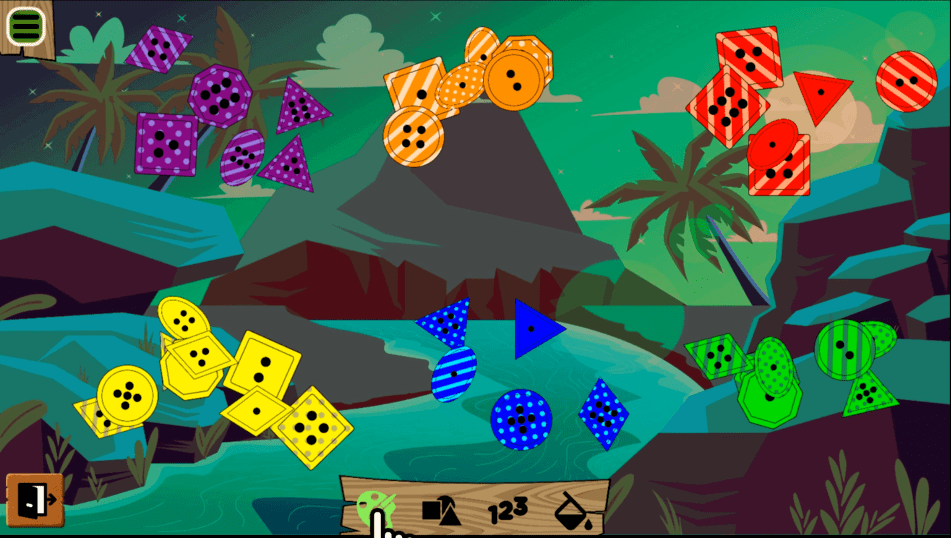
\includegraphics[width=1\textwidth]{figures/sortingscene2}
    \caption{Sorting Scene Category 1}
    \label{fig:sortingscene2}
\end{figure}

\begin{figure}[H]
    \centering
    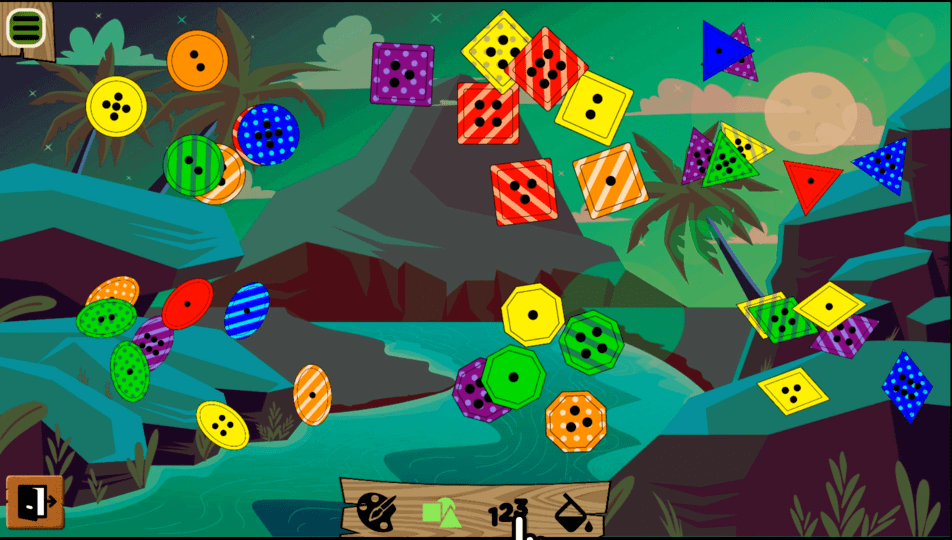
\includegraphics[width=1\textwidth]{figures/sortingscene3}
    \caption{Sorting Scene Category 2}
    \label{fig:sortingscene3}
\end{figure}

\begin{figure}[H]
    \centering
    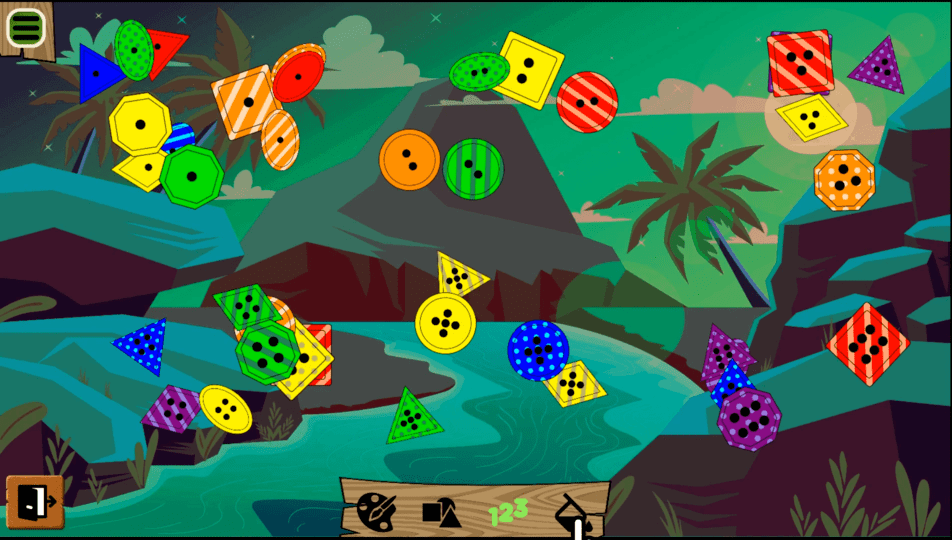
\includegraphics[width=1\textwidth]{figures/sortingscene4}
    \caption{Sorting Scene Category 3}
    \label{fig:sortingscene4}
\end{figure}

\begin{figure}[H]
    \centering
    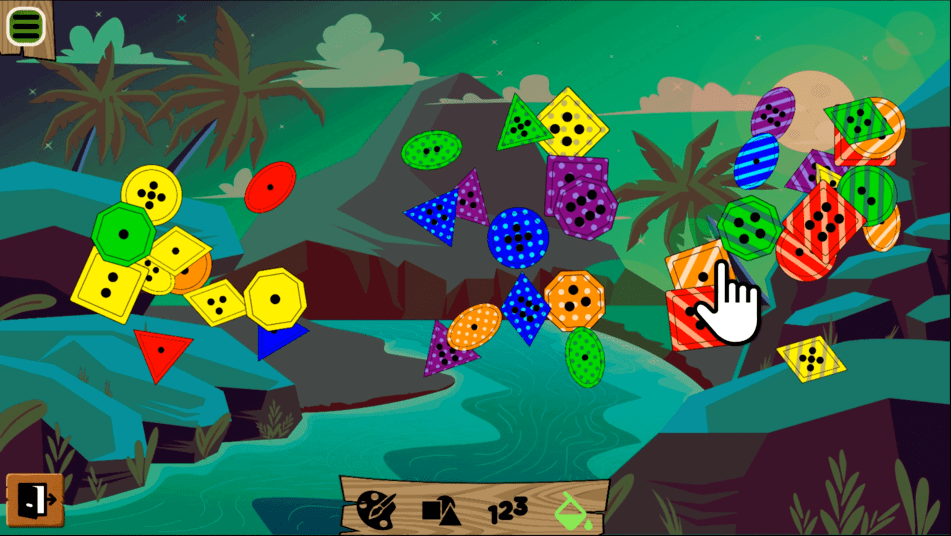
\includegraphics[width=1\textwidth]{figures/sortingscene5}
    \caption{Sorting Scene Category 4}
    \label{fig:sortingscene5}
\end{figure}

\begin{figure}[H]
    \centering
    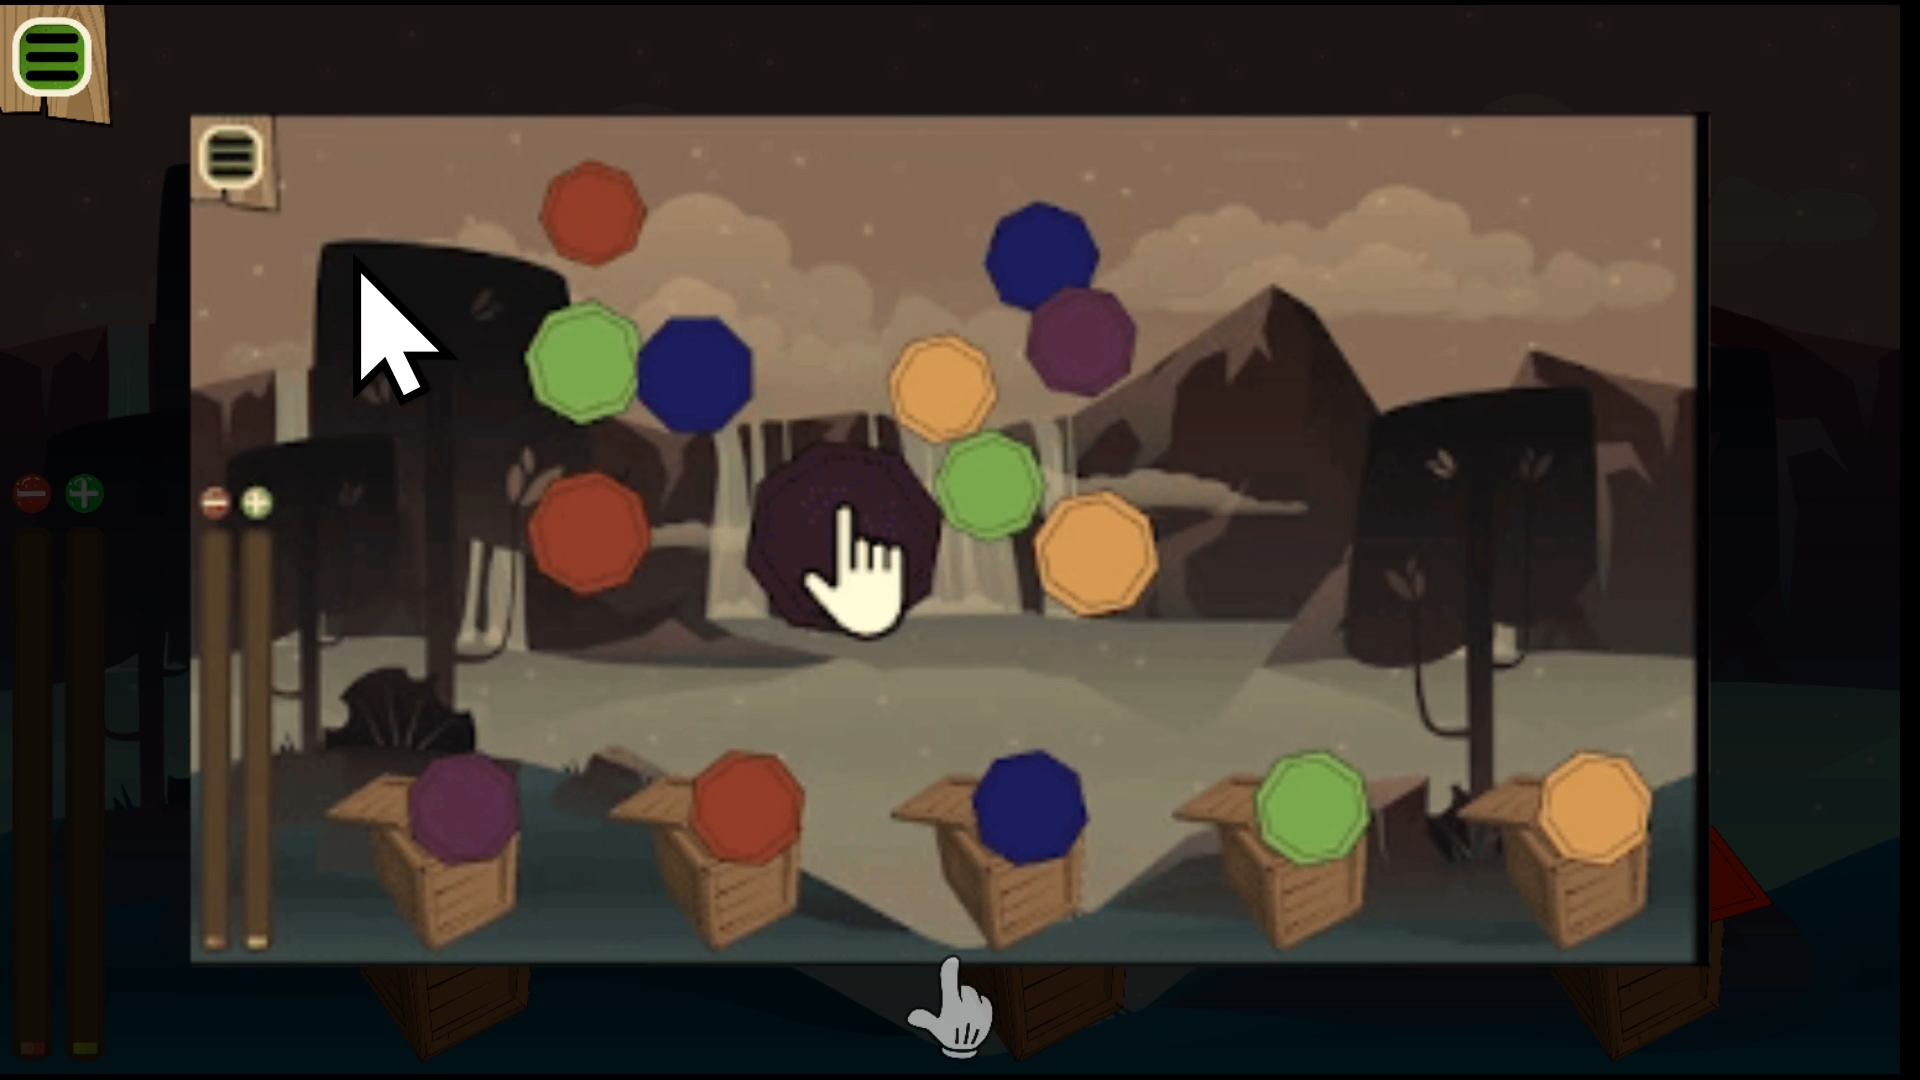
\includegraphics[width=1\textwidth]{figures/introduction}
    \caption{Introduction Screen to Sorting Scene}
    \label{fig:introduction}
\end{figure}

\begin{figure}[H]
    \centering
    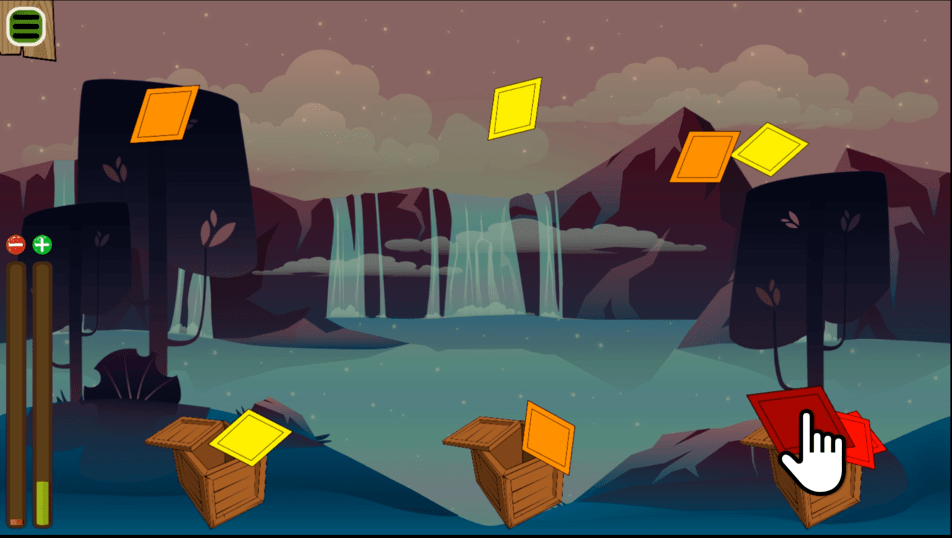
\includegraphics[width=1\textwidth]{figures/property1}
    \caption{Property Sorting Category 1}
    \label{fig:property1}
\end{figure}

\begin{figure}[H]
    \centering
    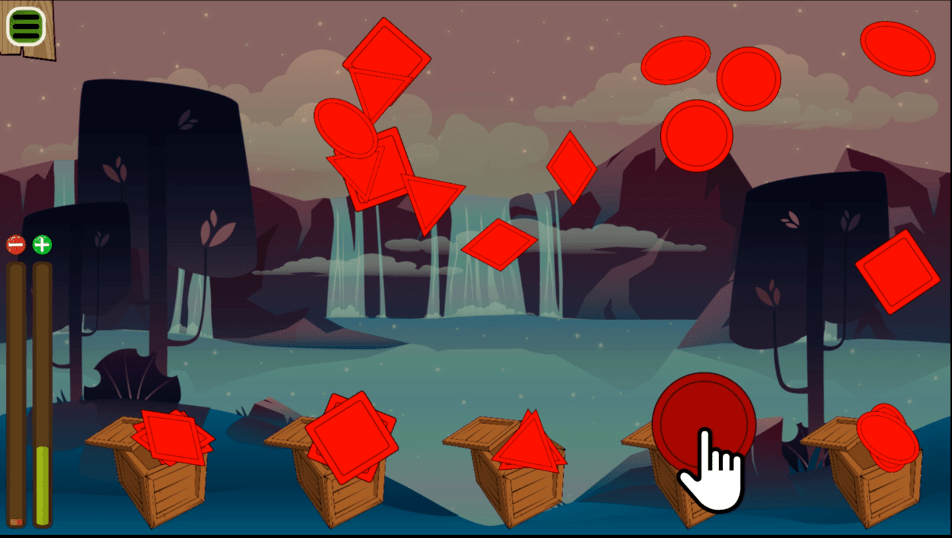
\includegraphics[width=1\textwidth]{figures/property2}
    \caption{Property Sorting Category 2}
    \label{fig:property2}
\end{figure}

\begin{figure}[H]
    \centering
    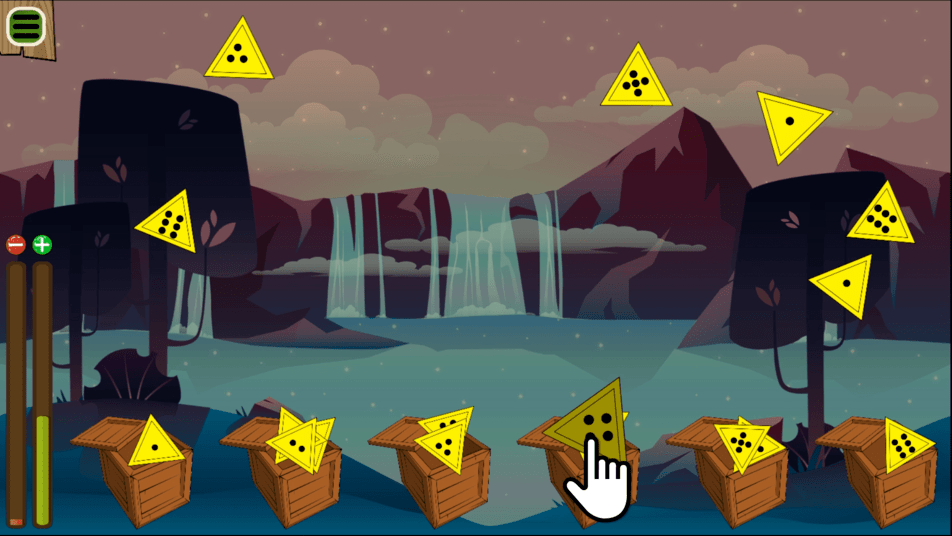
\includegraphics[width=1\textwidth]{figures/property3}
    \caption{Property Sorting Category 3}
    \label{fig:property3}
\end{figure}

\begin{figure}[H]
    \centering
    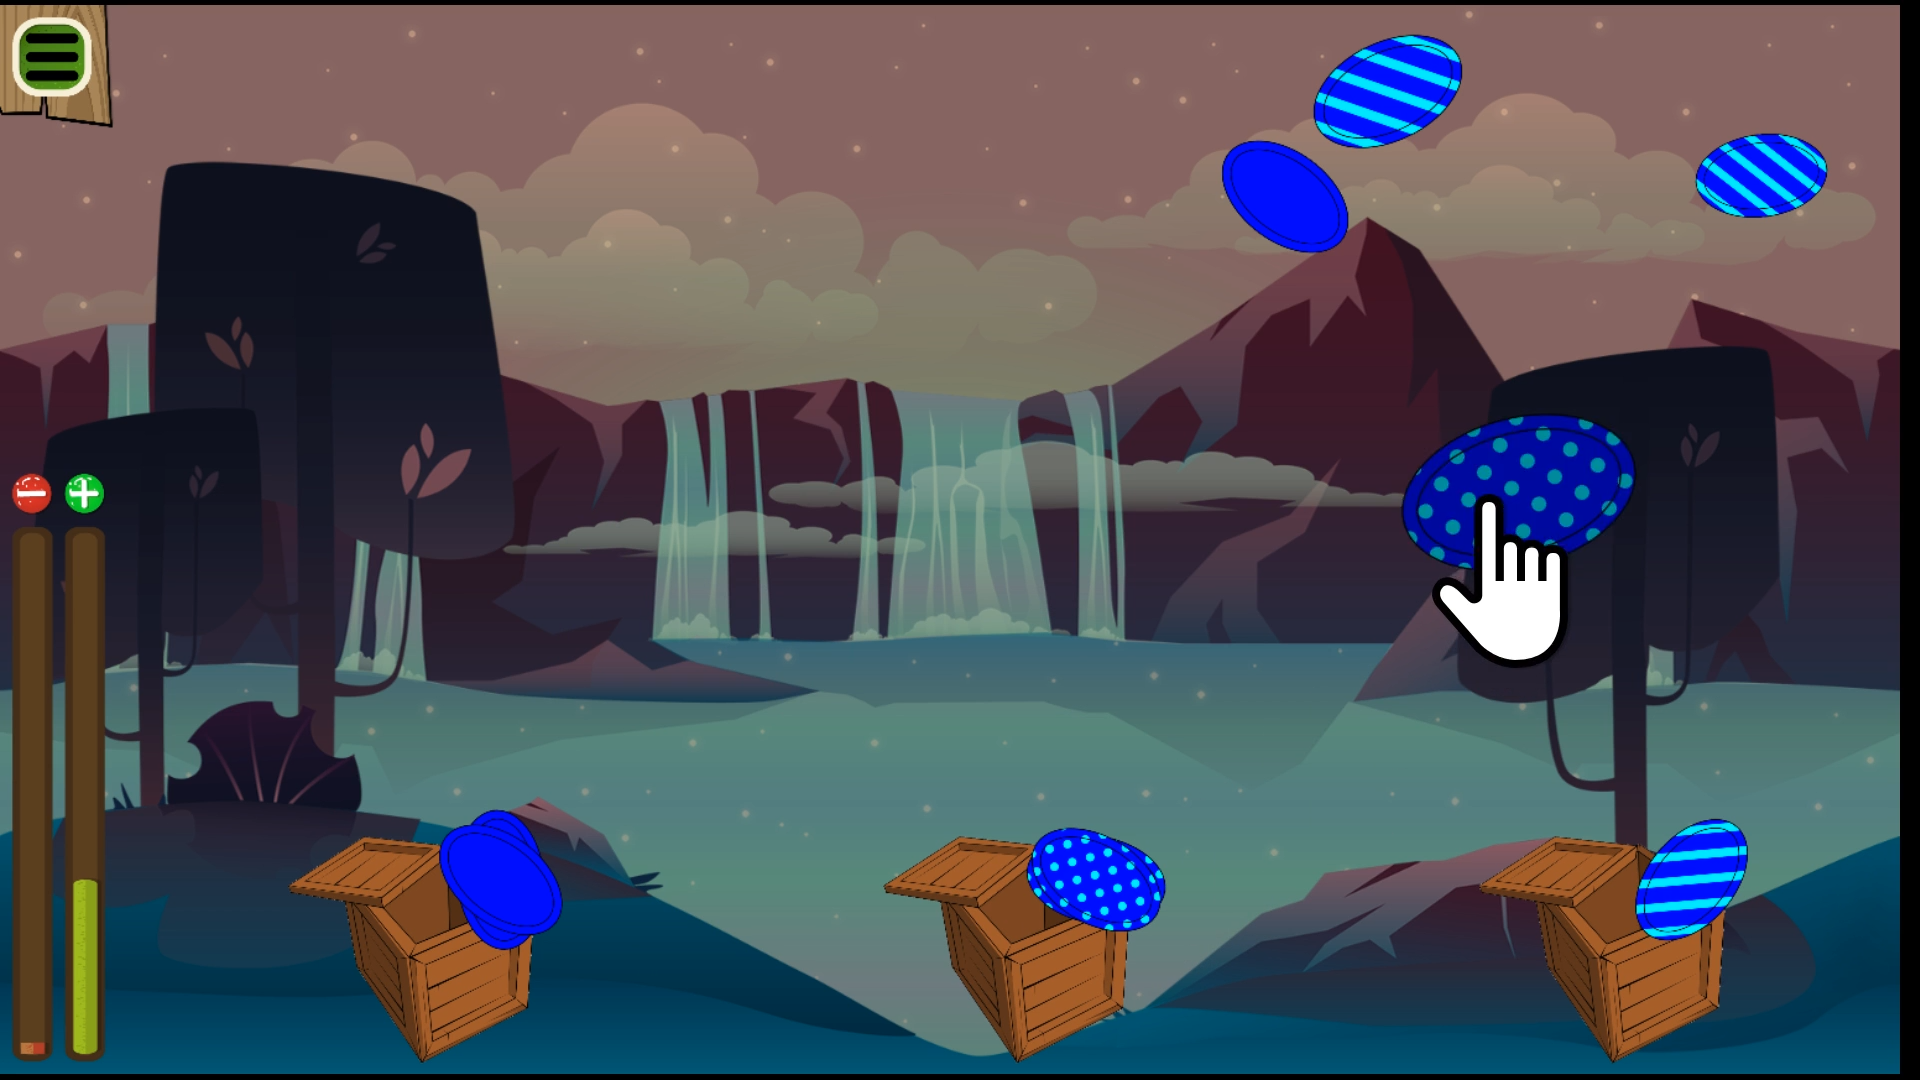
\includegraphics[width=1\textwidth]{figures/property4}
    \caption{Property Sorting Category 4}
    \label{fig:property4}
\end{figure}

\begin{figure}[H]
    \centering
    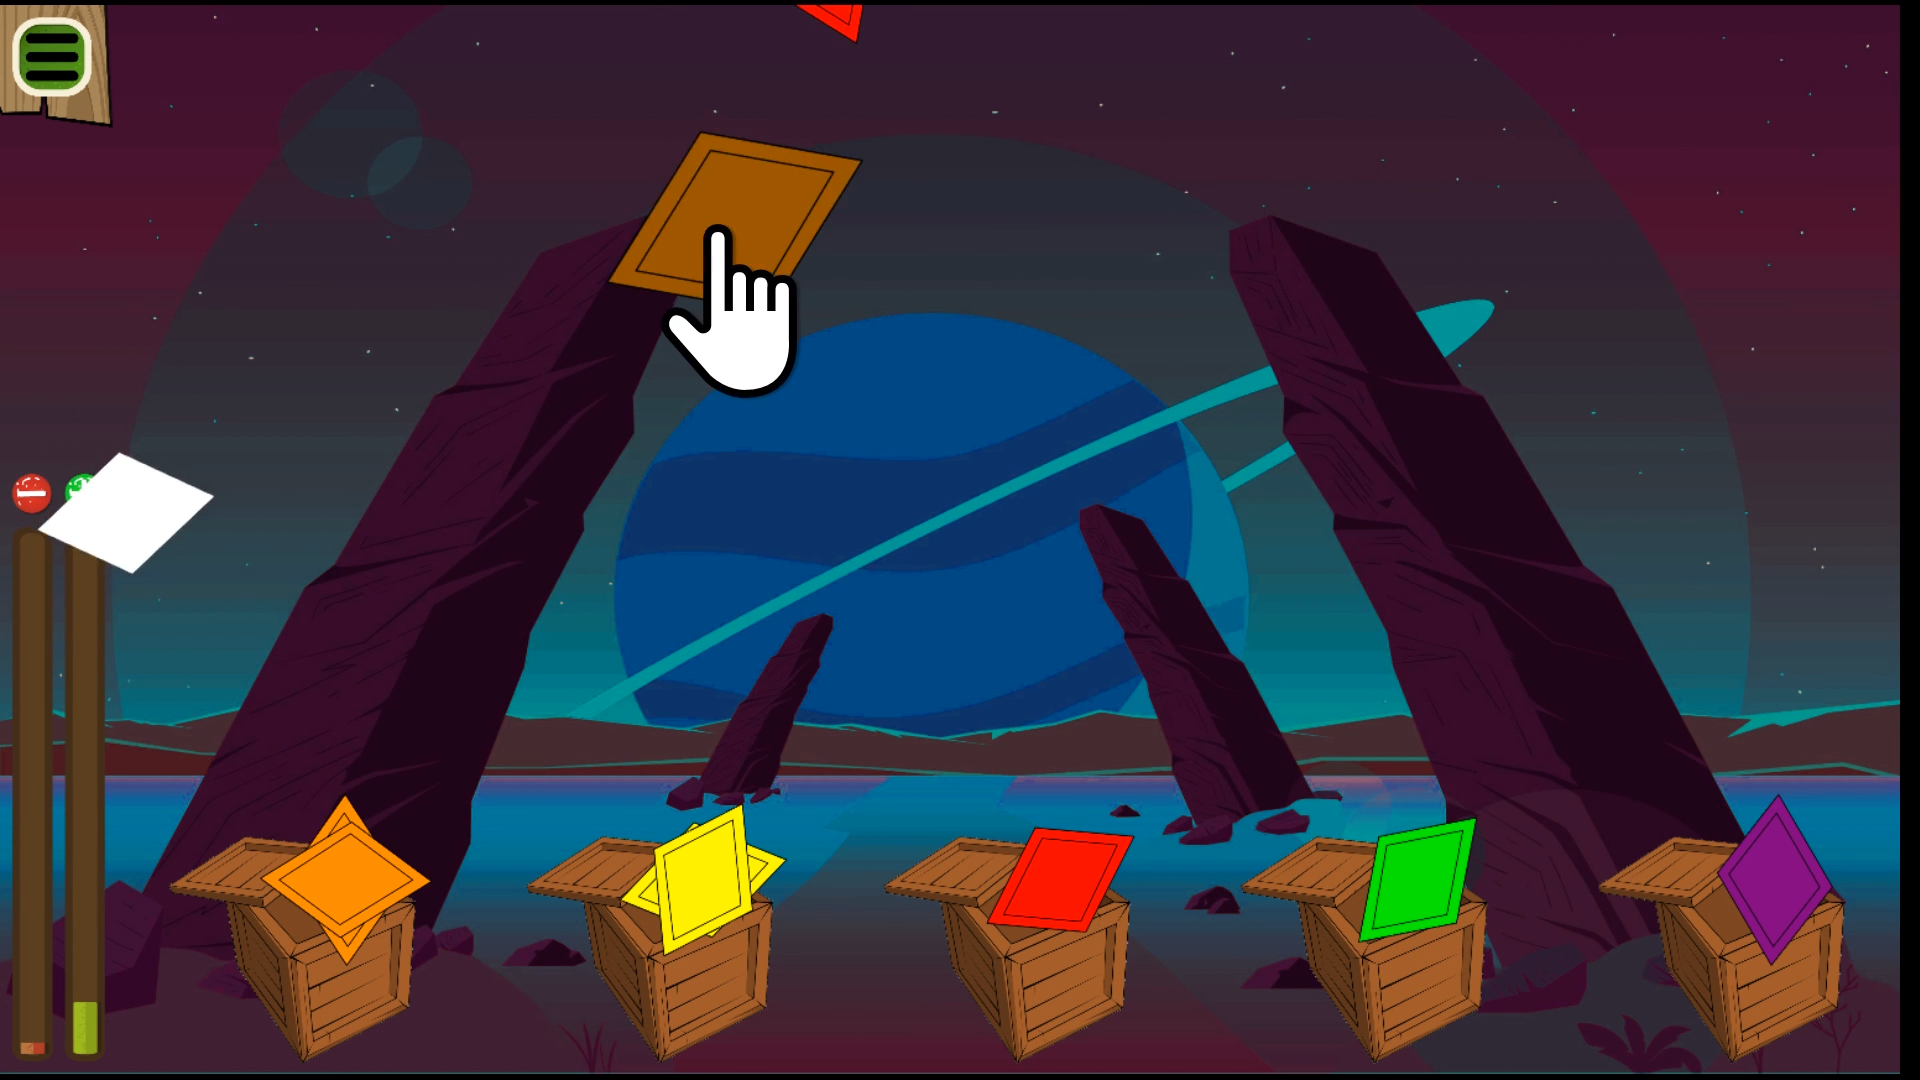
\includegraphics[width=1\textwidth]{figures/falling}
    \caption{Falling Property Sorting Category 1, 2-4 will be omitted}
    \label{fig:falling}
\end{figure}

\begin{figure}[H]
    \centering
    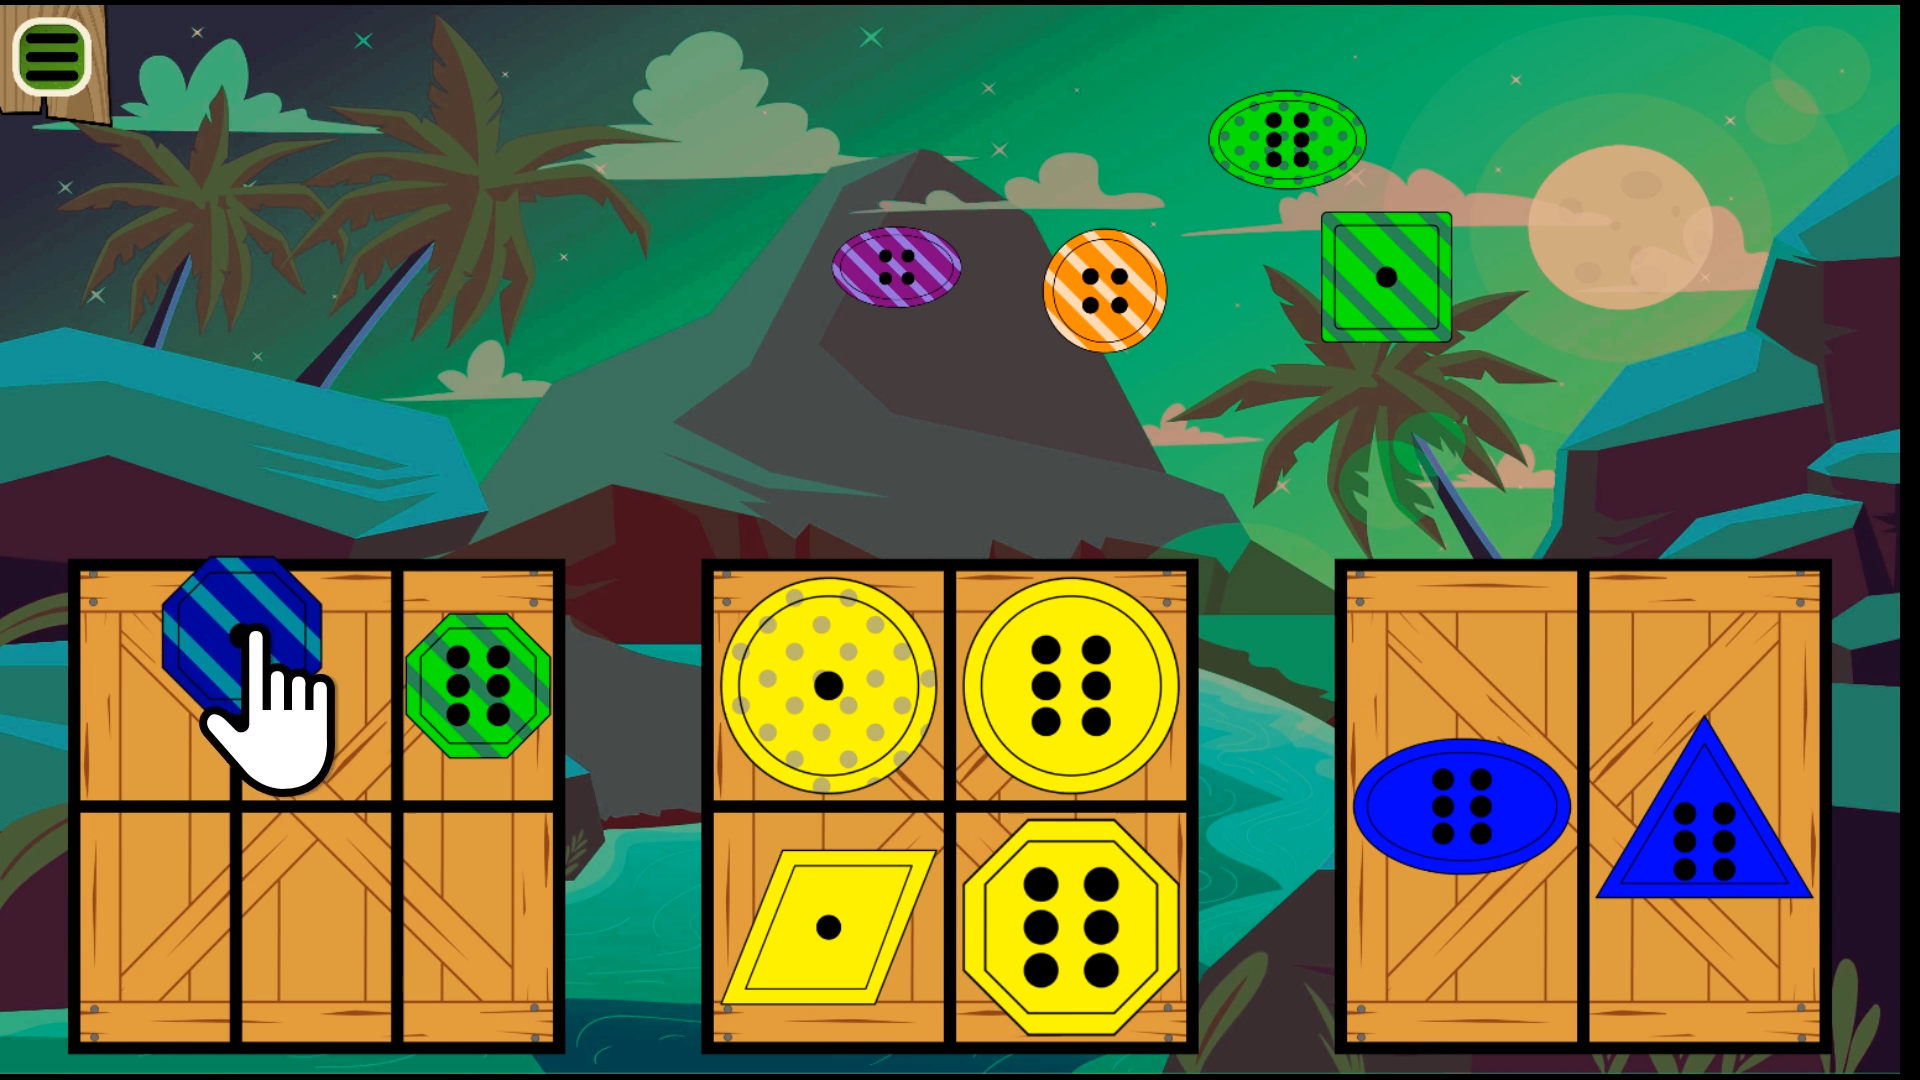
\includegraphics[width=1\textwidth]{figures/restricted1}
    \caption{Restricted Sorting Easy}
    \label{fig:restricted1}
\end{figure}

\begin{figure}[H]
    \centering
    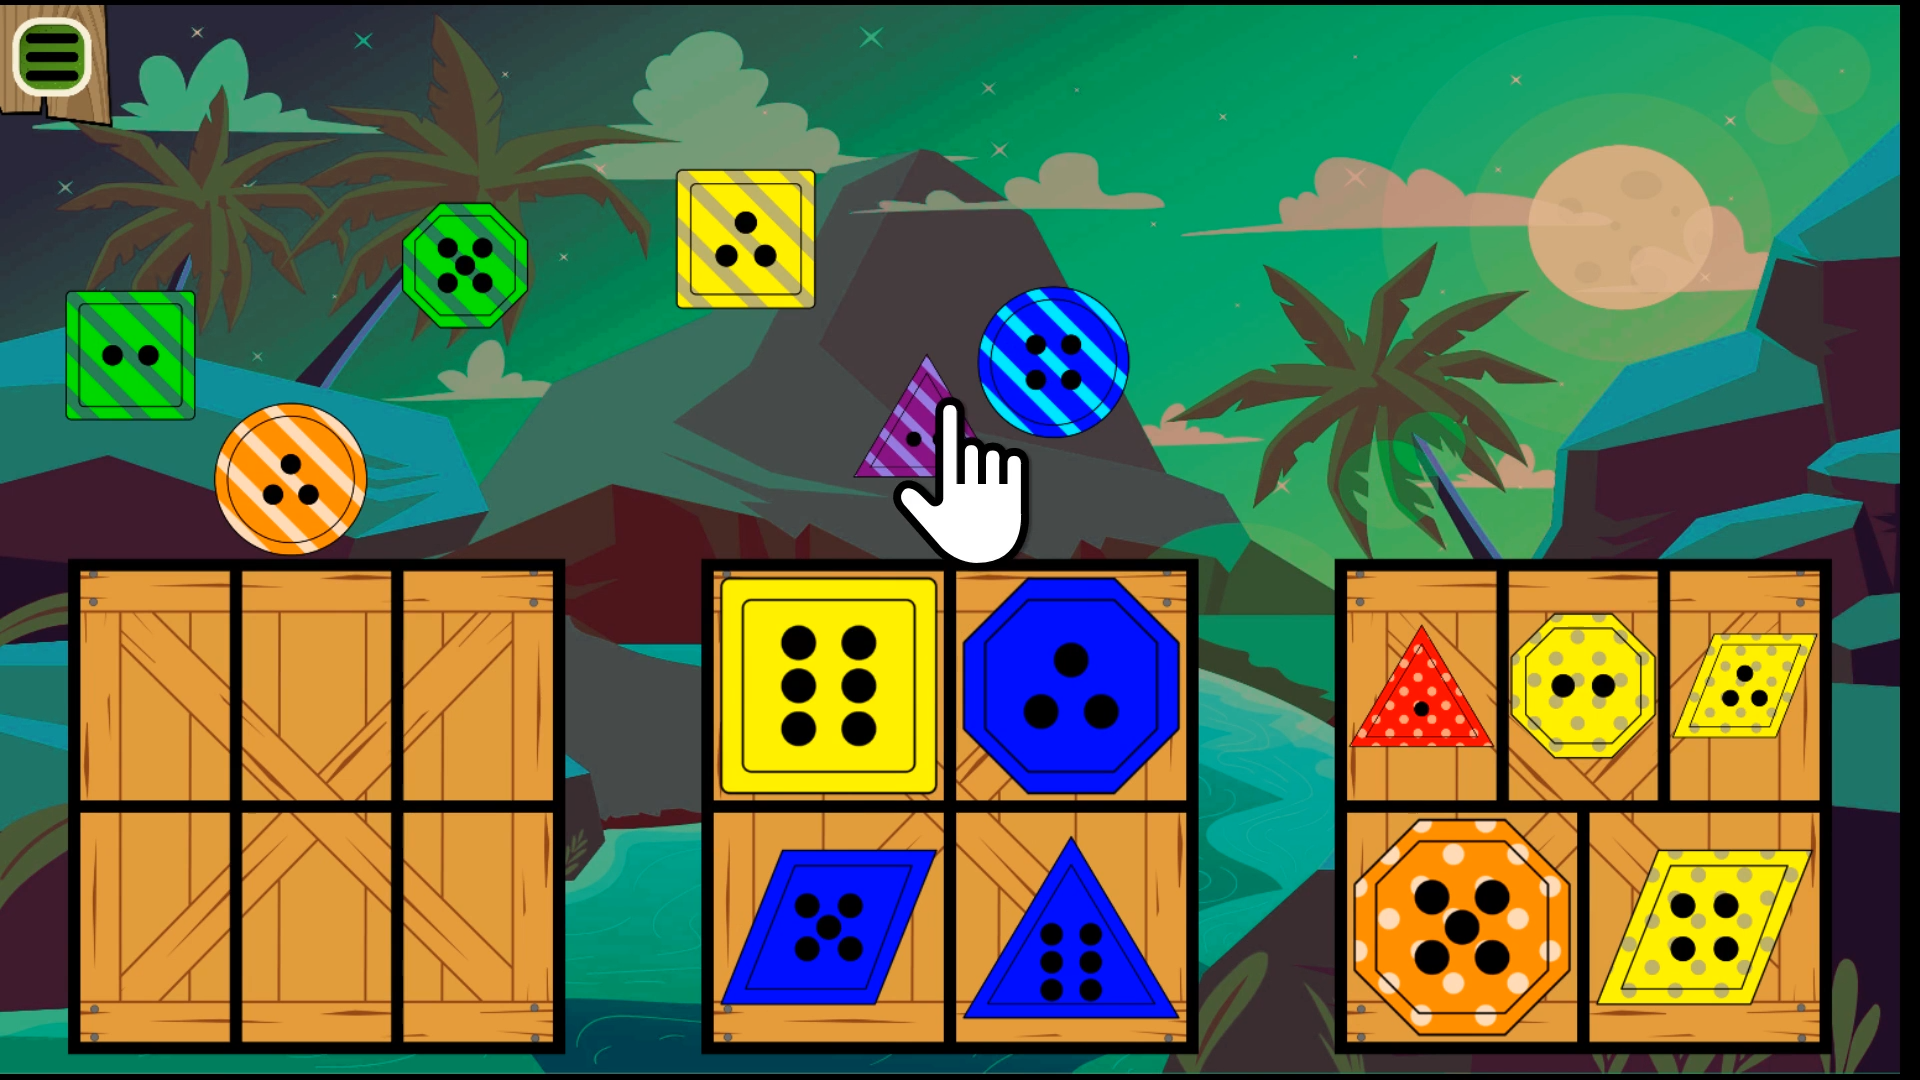
\includegraphics[width=1\textwidth]{figures/restricted2}
    \caption{Restricted Sorting 2 Hard}
    \label{fig:restricted2}
\end{figure}

\begin{figure}[H]
    \centering
    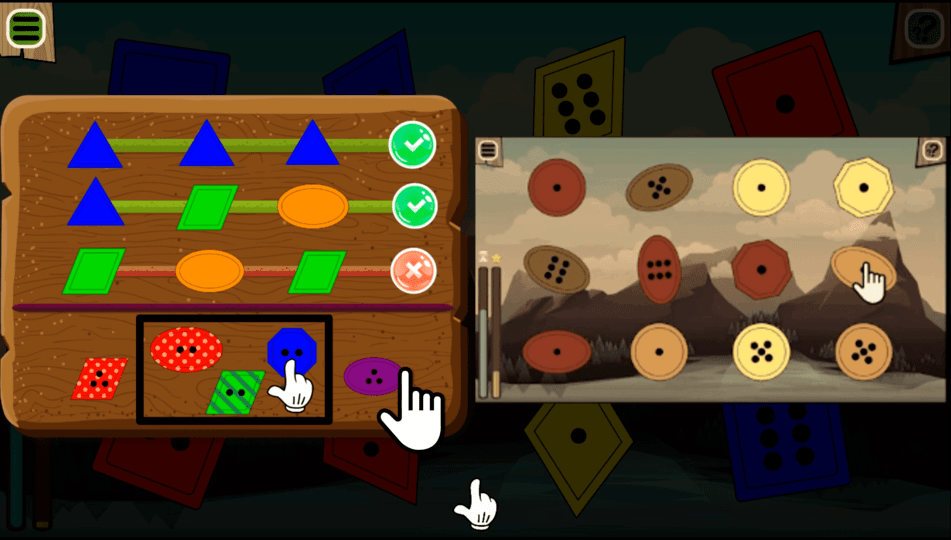
\includegraphics[width=1\textwidth]{figures/introgame}
    \caption{Introduction to Object Pairing Easy}
    \label{fig:introgame}
\end{figure}

\begin{figure}[H]
    \centering
    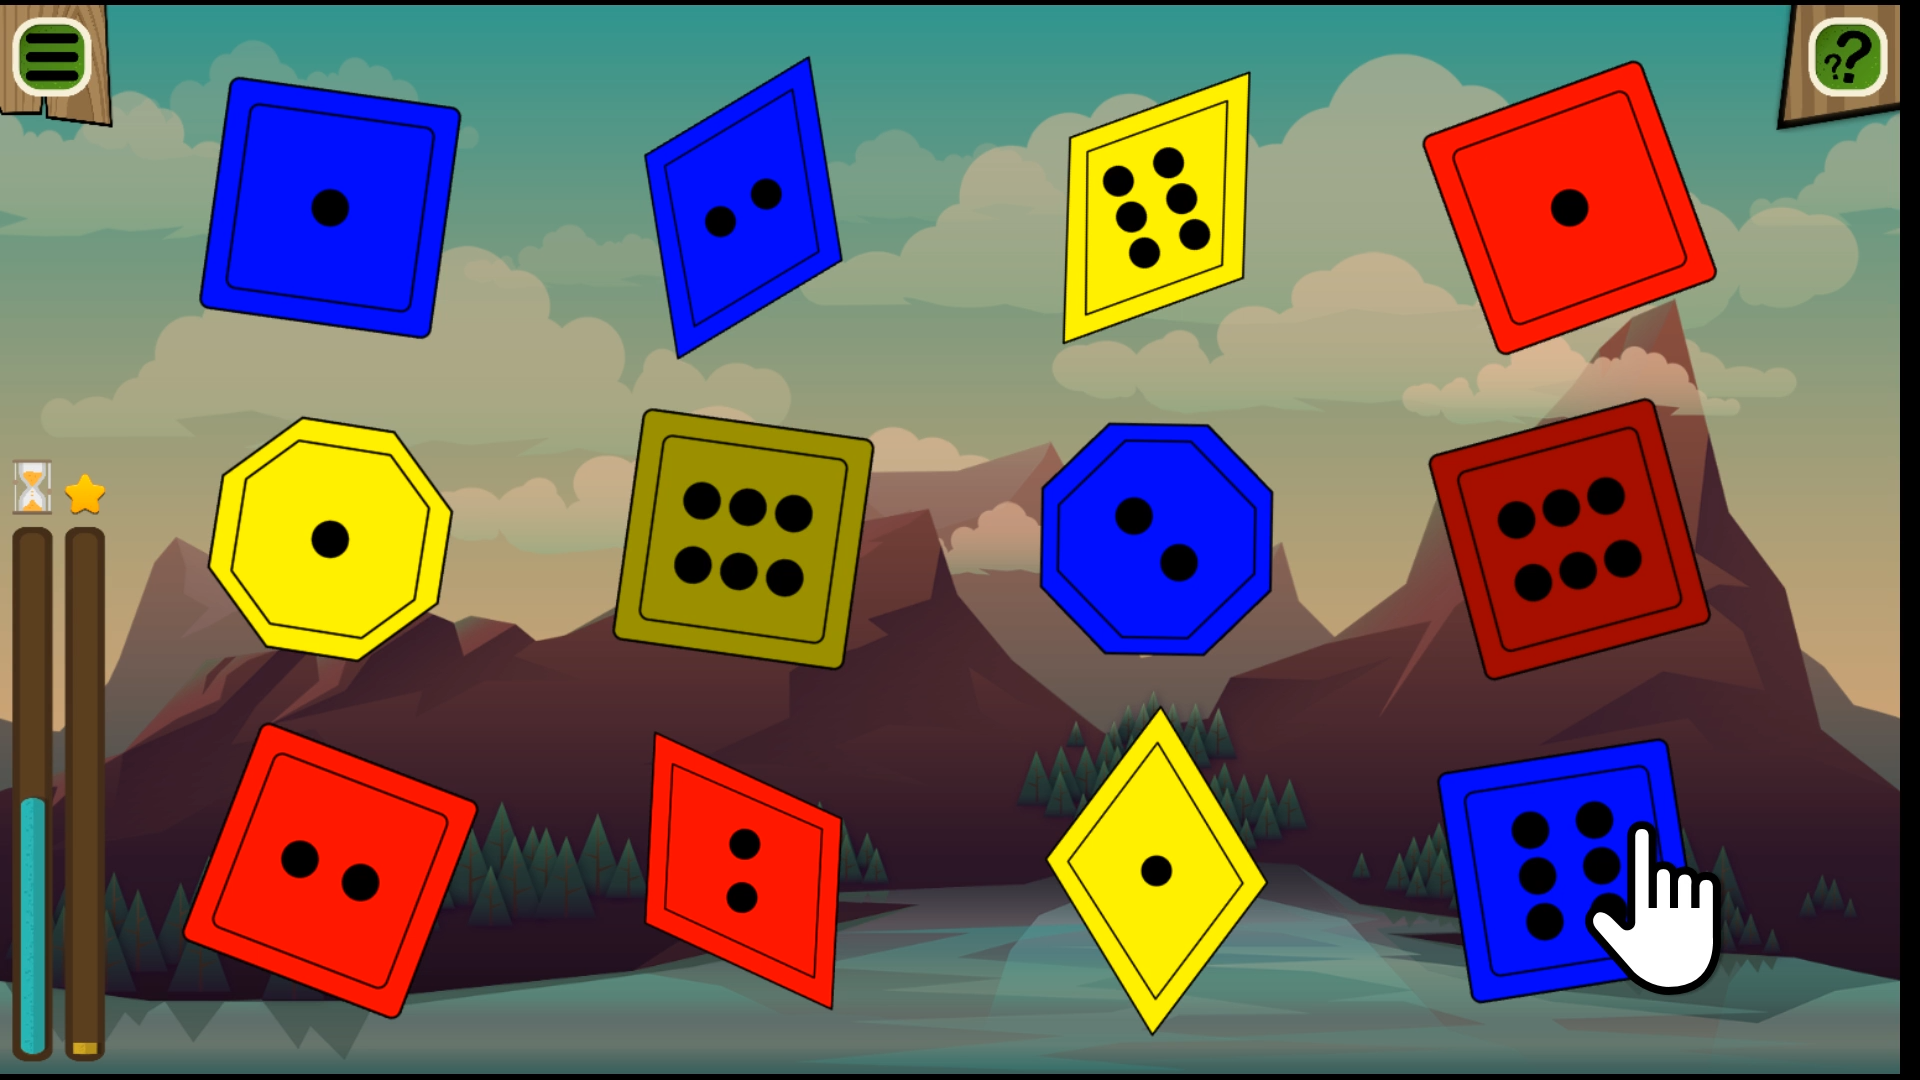
\includegraphics[width=1\textwidth]{figures/gameasy}
    \caption{Object Pairing Easy}
    \label{fig:gameeasy}
\end{figure}

\begin{figure}[H]
    \centering
    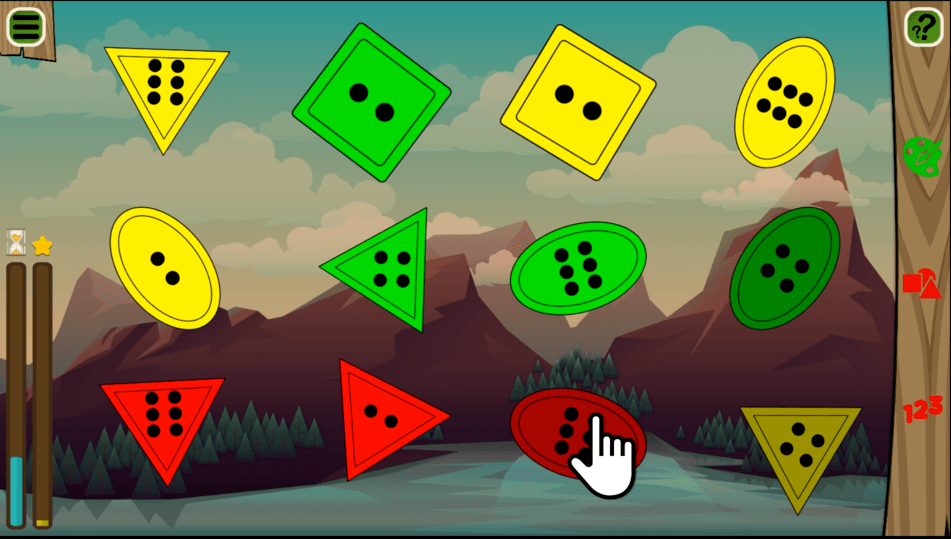
\includegraphics[width=1\textwidth]{figures/gameeasyhelp}
    \caption{Object Pairing Easy Helper Bar}
    \label{fig:gameeasyhelp}
\end{figure}

\begin{figure}[H]
    \centering
    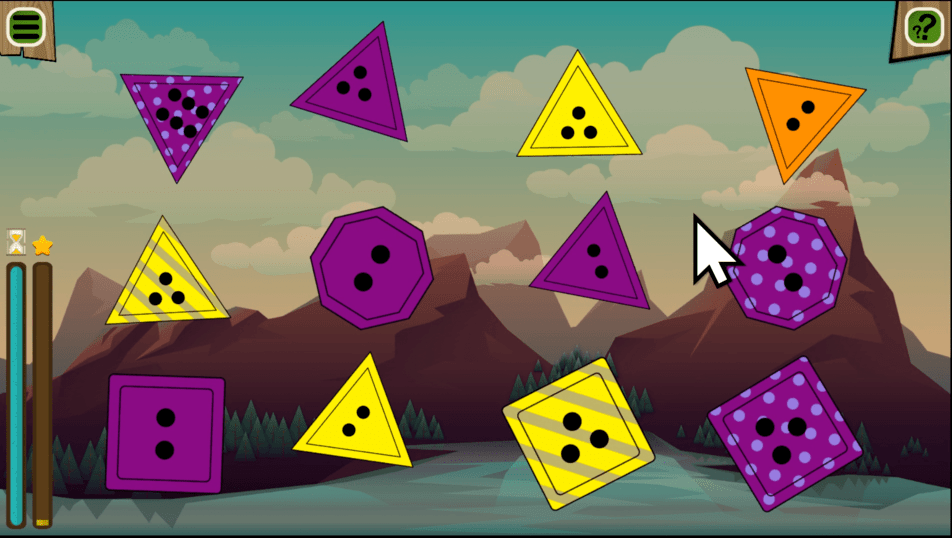
\includegraphics[width=1\textwidth]{figures/gamehard}
    \caption{Object Pairing Hard}
    \label{fig:gamehard}
\end{figure}

\begin{figure}[H]
    \centering
    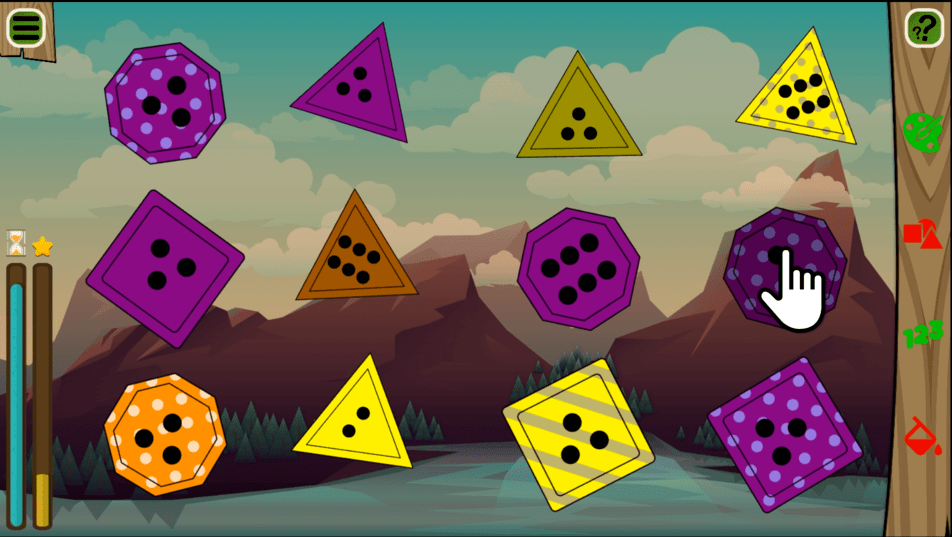
\includegraphics[width=1\textwidth]{figures/gamehardhelp}
    \caption{Object Pairing Hard Helper Bar}
    \label{fig:gamehardhelp}
\end{figure}

\begin{figure}[H]
    \centering
    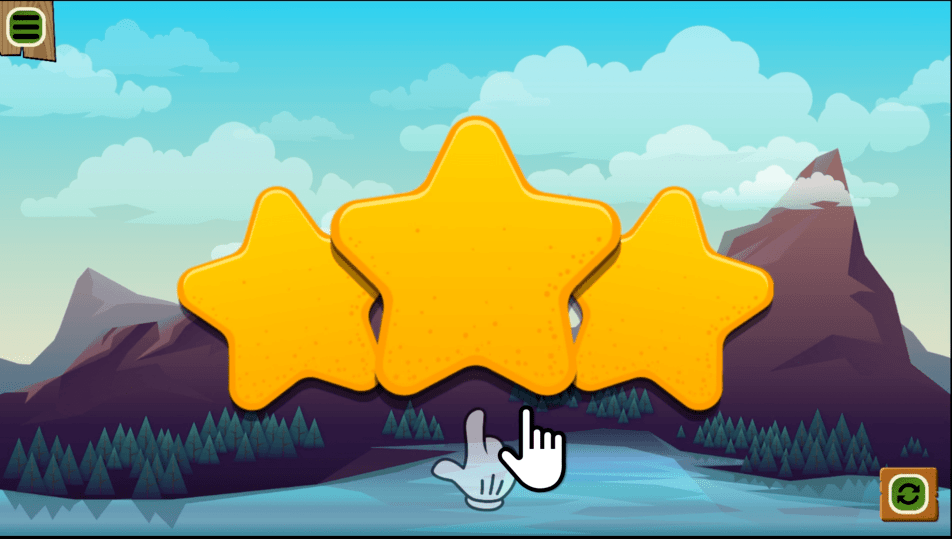
\includegraphics[width=1\textwidth]{figures/scorescreen}
    \caption{Score Screen}
    \label{fig:scorescreen}
\end{figure}
